\documentclass[12pt,a4]{article}
\usepackage{physics, amsmath,amsfonts,amsthm,amssymb, mathtools,steinmetz, gensymb, siunitx}	% LOADS USEFUL MATH STUFF
\usepackage{xcolor,graphicx}
\usepackage[left=45pt, top=20pt, right=45pt, bottom=45pt ,a4paper]{geometry} 				% ADJUSTS PAGE
\usepackage{setspace}
\usepackage{caption}
\usepackage{tikz}
\usepackage{pgf,tikz,pgfplots,wrapfig}
\usetikzlibrary{intersections}
\usepackage{tkz-euclide}
\usepackage{mathrsfs}
\usepackage{fancyhdr}
\usepackage{simpler-wick}
\usepackage{float}
\usepackage{array}
\usepackage{booktabs,multirow}
\usepackage{bm}
\usepackage{pst-node} 
%\usepackage{auto-pst-pdf}

\usetikzlibrary{decorations.text, calc}
\pgfplotsset{compat=1.7}

\usetikzlibrary{decorations.pathreplacing,decorations.markings}
\usepgfplotslibrary{fillbetween}
\allowdisplaybreaks

\newcommand{\vect}[1]{\boldsymbol{#1}}

\usepackage{hyperref}
%\usepackage[style= ACM-Reference-Format, maxbibnames=6, minnames=1,maxnames = 1]{biblatex}
%\addbibresource{references.bib}

\hypersetup{
    colorlinks=true,
    linkcolor=blue,
    filecolor=magenta,      
    urlcolor=cyan,
    pdfpagemode=FullScreen,
    }

\title{
\textsc{QT Homework 2}
}
\author{\textsc{J L Gouws}
}
\date{\today
\\[1cm]}



\usepackage{graphicx}
\usepackage{array}
\usepackage[compat=1.1.0]{tikz-feynman}




\begin{document}
\thispagestyle{empty}

\maketitle

%\feynmandiagram [horizontal=a to b] {
%  i1 -- [plain] a -- [plain] i2,
%  a -- [plain] b,
%  f1 -- [plain] b -- [plain] f2,
%};

\begin{enumerate}
  \item
    \begin{enumerate}
      \item 
        The only rule that changes is the interaction one:\\
        1. For each line
          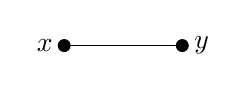
\begin{tikzpicture}[baseline={(current bounding box.center)}]
            \begin{feynman}
              \vertex [dot] (a) {};
              \vertex [dot, right=of a] (b) {};
              \diagram * {
                (a) -- [plain] (b),
              };
              \vertex [left= 0.7em of a] {$x$};
              \vertex [right= 0.7em of b] {$y$};
            \end{feynman}
          \end{tikzpicture} = $\Delta^{\phi}_F(x - y)$, and
          for each line
          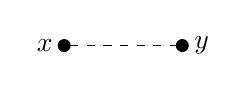
\begin{tikzpicture}[baseline={(current bounding box.center)}]
            \begin{feynman}
              \vertex [dot] (a) {};
              \vertex [dot, right=of a] (b) {};
              \diagram * {
                (a) -- [dashed] (b),
              };
              \vertex [left= 0.7em of a] {$x$};
              \vertex [right= 0.7em of b] {$y$};
            \end{feynman}
          \end{tikzpicture} = $\Delta^{\Phi}_F(x - y)$.
          
        2. Each external point gets a factor of one.

        3.
        For every vertex:
        \begin{center}
          \begin{tikzpicture}[baseline={(current bounding box.center)}]
            \begin{feynman}
              \vertex [dot] (a) {} ;
              \vertex [above left=of a] (i1) ;
              \vertex [above right=of a] (i2) ;
              \vertex [below=of a] (i3) ;
              \diagram * {
                (i1) -- [plain] (a) -- [plain] (i2),
                (a) -- [dashed] (i3),
              };
              \vertex [above= 0.7em of a] {$x$};
            \end{feynman}
          \end{tikzpicture}
        \end{center}
        Associate a factor of:
        \begin{equation*}
          -ig\int d^4x
        \end{equation*}
        4. Divide by the symmetry factor.
      \item
        The diagrams are:\\
        \begin{center}
          \begin{tikzpicture}[baseline={(current bounding box.center)}]
            \begin{feynman}
              \vertex [dot] (a) {} ;
              \vertex [above left=of a, dot] (i1) {};
              \vertex [above right=of a, dot] (i2) {};
              \vertex [below=of a,dot] (i3) {};
              \diagram * {
                (i1) -- [plain] (a) -- [plain] (i2),
                (a) -- [dashed] (i3),
              };
              \vertex [below left = 0.7em of a] {$q$};
              \vertex [above= 0.7em of i1] {$z$};
              \vertex [above= 0.7em of i2] {$y$};
              \vertex [below= 0.7em of i3] {$x$};
            \end{feynman}
          \end{tikzpicture}
        \end{center}

        This has the associated integral:
        \begin{equation*}
          -ig\int d^4 q\Delta^{\Phi}_{xq} \Delta^{\varphi}_{yq}\Delta^{\varphi}_{zq}
        \end{equation*}

        \begin{center}
          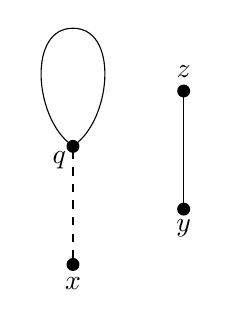
\begin{tikzpicture}[baseline={(current bounding box.center)}]
            \begin{feynman}
              \vertex [dot] (a) {};
              \vertex [above of = a] (b) ;
              \vertex [above right = 2em and 4em of a, dot] (i1) {};
              \vertex [below=of i1, dot] (i2) {};
              \vertex [below=of a,dot] (i3) {};
              \diagram * {
                (i1) -- [plain] (i2),
                (i3) -- [dashed] (a) -- [out=40, in=0, min distance=0.5cm] (b) -- [out=180, in=140, min distance=0.5cm] (a),
  %                (a) -- [out=45, in=-45, loop, min distance=2cm] (a),%-- [plain, half left] (b) -- [plain, half left] (a),
              };
  %              \draw (a) arc [start angle=0, end angle=-180, radius=0.7cm];
              \vertex [below left = 0.7em of a] {$q$};
              \vertex [above= 0.7em of i1] {$z$};
              \vertex [below= 0.7em of i2] {$y$};
              \vertex [below= 0.7em of i3] {$x$};
            \end{feynman}
          \end{tikzpicture}
        \end{center}

        This has the associated integral:
        \begin{equation*}
          -\frac{ig}{2}\Delta^{\varphi}_{yz}\int d^4 q\Delta^{\Phi}_{xq} \Delta^{\varphi}_{qq}
        \end{equation*}
      \item
        \begin{enumerate}
          \item
            Taking the fourier transform of:
            \begin{equation*}
              G_1(x, y, z) = -ig\int d^4 q\Delta^{\Phi}_{xq} \Delta^{\varphi}_{yq}\Delta^{\varphi}_{zq}
            \end{equation*}
            Gives:\footnote{The definition of the propagator has a $(2\pi)^4$ in the denominator which will cancel out the extra ones.}
            \begin{align*}
              \tilde G_1(p_1, p_2, p_3) &= -ig\int d^4x e^{-i p_1\cdot x}\int d^4y e^{-i p_2\cdot y}\int d^4z e^{-i p_3\cdot z}\int d^4 q\Delta^{\Phi}_{xq} \Delta^{\varphi}_{yq}\Delta^{\varphi}_{zq}\\
                                        &= -ig\int d^4x e^{-i p_1 \cdot x}\int d^4y e^{-i p_2\cdot y}\\
                                        & \qquad \times \int d^4z e^{-i p_3\cdot z}\int d^4 q\int \frac{d^4 k}{(2 \pi)^4} \frac{e^{ik\cdot (x - q)}}{k^2 - M^2 + i \epsilon} \Delta^{\varphi}_{yq}\Delta^{\varphi}_{zq}\\
                                        &= -ig\int d^4y e^{-i p_2\cdot y}\int d^4z e^{-i p_3\cdot z}\int d^4 q\\
                                        & \qquad \times \int \frac{d^4 k}{(2 \pi)^4} \frac{e^{-ik\cdot  q}}{k^2 - M^2 + i \epsilon}\left[\int d^4x e^{i(k - p_1)\cdot x} \right]\Delta^{\varphi}_{yq}\Delta^{\varphi}_{zq}\\
                                        &= -ig\int d^4y e^{-i p_2\cdot y}\int d^4z e^{-i p_3\cdot z}\int d^4 q\\
                                        &\qquad \times \left[\int d^4 k \frac{e^{-ik\cdot  q}\delta^{(4)}(k - p_1)}{k^2 - M^2 + i \epsilon}\right] \Delta^{\varphi}_{yq}\Delta^{\varphi}_{zq}\\
                                        &= -ig\int d^4y e^{-i p_2\cdot y}\int d^4z e^{-i p_3\cdot z}\int d^4 q \frac{e^{-ip_1\cdot  q}}{p_1^2 - M^2 + i \epsilon} \Delta^{\varphi}_{yq}\Delta^{\varphi}_{zq}\\
                                        &= -ig \int d^4 q \frac{e^{-ip_1\cdot  q}}{p_1^2 - M^2 + i \epsilon} \frac{e^{-ip_2\cdot  q}}{p_2^2 - m^2 + i \epsilon}\frac{e^{-ip_3\cdot  q}}{p_3^2 - m^2 + i \epsilon}\\
                                        &= -ig (2 \pi)^{4} \frac{1}{p_1^2 - M^2 + i \epsilon} \frac{1}{p_2^2 - m^2 + i \epsilon}\frac{1}{p_3^2 - m^2 + i \epsilon}\delta^{(4)}(p_1 + p_2 + p_3)\\
            \end{align*}
            This seems weird with all the $(2\pi)$ factors, that come with the deltas as integrals over the complex exponentials.
            The fourier transform of
            \begin{equation*}
               G_2(x, y, z) = -\frac{ig}{2}\Delta^{\varphi}_{yz}\int d^4 q\Delta^{\Phi}_{xq} \Delta^{\varphi}_{qq}
            \end{equation*}
            is
            \begin{align*}
              \tilde G_2(p_1, p_2, p_3) &= -\frac{ig}{2}\int d^4x e^{-i p_1\cdot x}\int d^4y e^{-i p_2\cdot y}\int d^4z e^{-i p_3\cdot z}\Delta^{\varphi}_{yz}\int d^4 q\Delta^{\Phi}_{xq} \Delta^{\varphi}_{qq}\\
                                        &= -\frac{ig}{2}\frac{1}{p_1^2 - M^2 + i \epsilon} \int d^4y e^{-i p_2\cdot y}\int d^4z e^{-i p_3\cdot z}\Delta^{\varphi}_{zy}\int d^4 q e^{-ip_1\cdot  q} \Delta^{\varphi}_{qq}\\
                                        &= -\frac{ig}{2}\frac{1}{p_1^2 - M^2 + i \epsilon} \int d^4 k\frac{\delta^{(4)}(k - p_2)\delta^{(4)}(k - p_3)}{k^2 - m^2 + i \epsilon}\\
                                        & \qquad \times \int d^4 q e^{-ip_1\cdot  q} \Delta^{\varphi}_{qq}\\
                                        &= -\frac{ig}{2}\frac{1}{p_1^2 - M^2 + i \epsilon} \frac{\delta^{(4)}(p_2 - p_3)}{p_2^2 - m^2 + i \epsilon}\int d^4 q e^{-ip_1\cdot  q} \Delta^{\varphi}_{qq}\\
                                        &= -\frac{ig}{2}\frac{1}{p_1^2 - M^2 + i \epsilon} \frac{\delta^{(4)}(p_2 - p_3)}{p_2^2 - m^2 + i \epsilon}\int d^4 q e^{-ip_1\cdot  q} \int d^4k\frac{e^0}{k^2 - m^2 + i \epsilon}\\
                                        &= -\frac{ig}{2}\frac{1}{p_1^2 - M^2 + i \epsilon} \frac{\delta^{(4)}(p_2 - p_3)}{p_2^2 - m^2 + i \epsilon}\left[ \int d^4 q e^{-ip_1\cdot  q}\right]\int d^4k\frac{e^0}{k^2 - m^2 + i \epsilon}\\
                                        &= -\frac{ig}{2}\frac{1}{p_1^2 - M^2 + i \epsilon} \frac{\delta^{(4)}(p_2 - p_3)}{p_2^2 - m^2 + i \epsilon}(2\pi)^4\delta^{(4)}(p_1)\int d^4k\frac{1}{k^2 - m^2 + i \epsilon}
            \end{align*}
            Now this is physically zero, because for the $\Phi$ particle to exist it must have some energy implying $p_1^0 > 0$ and $\delta(p_1) = 0$.


          \item
            The form of the of the Fourier transform is nearly the same as the form of the LSZ reduction formula, the difference being the absence of the derivatives: $(\partial^2 - m^2)$.
            The action of derivative is to take it's Green's function (propagator) and turn it into a dirac delta.
            This analogy can be used to modify the rules for the matrix element $i \mathcal{M}$.
            In the previous calculation the fourier transform of propagator, gave a factor: $\frac{1}{p^2 - m^2 + i\epsilon}$.
            Therefore, I presume the momentum space greens functions go something like this:
            \begin{itemize}
              \item For every line associate a factor of $\frac{1}{p^2 - m^2 + i\epsilon}$.
              \item Each exernal line has a factor of $1$
              \item For every vertex associate a factor of $- i g (2 \pi)^4 \delta(\sum_p p)$.
              \item Divide by the symmetry factor.
            \end{itemize}
            Only the fully connected diagrams contribute to the Matrix element:\\
            \begin{center}
              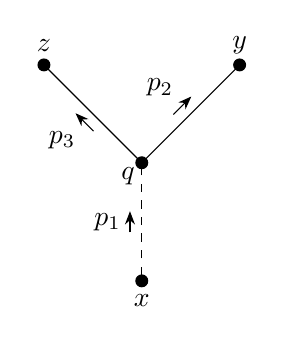
\begin{tikzpicture}[baseline={(current bounding box.center)},
                arrowlabel/.style={
                  /tikzfeynman/momentum/.cd, % means that the following keys are read from the /tikzfeynman/momentum family
                  arrow shorten=#1,arrow distance=1.5mm
                },
                arrowlabel/.default=0.4
                ]
                \begin{feynman}
                  \vertex [dot] (a) {} ;
                  \vertex [above left=5em of a, dot] (i1) {};
                  \vertex [above right=5em of a, dot] (i2) {};
                  \vertex [below=of a,dot] (i3) {};
                  \diagram * {
                    (a) -- [plain, momentum={[arrowlabel]$p_3$}] (i1),
                    (a) -- [plain, momentum={[arrowlabel]$p_2$}] (i2),
                    (i3) -- [dashed, momentum={[arrowlabel]$p_1$}] (a),
                  };
                  \vertex [below left = 0.7em of a] {$q$};
                  \vertex [above= 0.7em of i1] {$z$};
                  \vertex [above= 0.7em of i2] {$y$};
                  \vertex [below= 0.7em of i3] {$x$};
                \end{feynman}
            \end{tikzpicture}
            \end{center}

            Applying the rules gives:
              \begin{equation*}
              \tilde G_1(p_1, p_2, p_3) = -ig (2 \pi)^{4} \frac{1}{p_1^2 - M^2 + i \epsilon} \frac{1}{p_2^2 - m^2 + i \epsilon}\frac{1}{p_3^2 - m^2 + i \epsilon}\delta^{(4)}(p_1 + p_2 + p_3)\\
              \end{equation*}
              It is clear that the momentum rules for the Green's function and the matrix element are different, but closely related.
              The same, only fully connected, diagrams contribute.
        \end{enumerate}
      \item
        From the LSZ formula:
        \begin{align*}
          \langle f | S | i \rangle &= -ig\int d^4x \int d^4y \int d^4z e^{i(p \cdot x - k_1 \cdot y - k_2 \cdot z)} (\partial_x^2 + M^2)(\partial_y^2 + m^2)(\partial_z^2 + m^2) \\
                                    & \qquad \times \int d^4 q\Delta^{\Phi}_{xq} \Delta^{\varphi}_{yq}\Delta^{\varphi}_{zq}\\
                                    &= -ig \int d^4x \int d^4y \int d^4z e^{i(p \cdot x - k_1 \cdot y - k_2 \cdot z)} \int d^4 q  (\partial_x^2 + M^2) \Delta^{\Phi}_{xq} (\partial_y^2 + m^2)(\partial_z^2 + m^2) \\
                                    & \qquad \times  \Delta^{\varphi}_{yq}\Delta^{\varphi}_{zq}\\
                                    &= -ig \int d^4x \int d^4y \int d^4z e^{i(p \cdot x - k_1 \cdot y 0 k_2 \cdot z)} \int d^4 q \delta^4(x - q) (\partial_y^2 + m^2)(\partial_z^2 + m^2) \\
                                    & \qquad \times  \Delta^{\varphi}_{yq}\Delta^{\varphi}_{zq}\\
                                    &= -ig \int d^4x \int d^4y \int d^4z e^{i(p \cdot x - k_1 \cdot y - k_2 \cdot z)} (\partial_y^2 + m^2)(\partial_z^2 + m^2) \Delta^{\varphi}_{yx}\Delta^{\varphi}_{zx}\\
                                    &= -ig \int d^4y \int d^4z e^{i(p \cdot y - k_1 \cdot y - k_2 \cdot z)} (\partial_z^2 + m^2) \Delta^{\varphi}_{zy}\\
                                    &= -ig \int d^4y \int d^4z e^{i(p \cdot y - k_1 \cdot y - k_2 \cdot z)} \delta^4(z - y)\\
                                    &= -ig \int d^4y e^{i(p  - k_1 - k_2)\cdot y} \\
                                    &= -ig (2 \pi)^4 \delta^4(p  - k_1 - k_2)
        \end{align*}
        The question asks for next to leading order, so it seems to require the next term in the Dyson series which will be a term of order $g^3$:
            \begin{center}
              \begin{tikzpicture}[baseline={(current bounding box.center)},
                arrowlabel/.style={
                  /tikzfeynman/momentum/.cd, % means that the following keys are read from the /tikzfeynman/momentum family
                  arrow shorten=#1,arrow distance=1.5mm
                },
                arrowlabel/.default=0.4
                ]
                \begin{feynman}
                  \vertex [dot] (a) {} ;
                  \vertex [above left=5em of a, dot] (i1) {};
                  \vertex [above right=5em of a, dot] (i2) {};
                  \vertex [above left=5em of i1, dot] (i3) {};
                  \vertex [above right=5em of i2, dot] (i4) {};
                  \vertex [below=of a,dot] (i5) {};
                  \diagram * {
                    (i3) -- [plain] (i1),
                    (i2) -- [plain] (i4),
                    (a) -- [plain] (i1),
                    (a) -- [plain] (i2),
                    (i5) -- [dashed] (a),
                    (i1) -- [dashed] (i2),
                  };
                  \vertex [below left = 0.7em of a] {$q$};
                  \vertex [below left= 0.7em of i1] {$r$};
                  \vertex [below right= 0.7em of i2] {$s$};
                  \vertex [above= 0.7em of i4] {$z$};
                  \vertex [above= 0.7em of i3] {$y$};
                  \vertex [below= 0.7em of i5] {$x$};
                \end{feynman}
            \end{tikzpicture}
            \end{center}
            This has the expression:
        \begin{align*}
          \langle f | S | i \rangle &= ig^3\int d^4x \int d^4y \int d^4z e^{i(p \cdot x - k_1 \cdot y - k_2 \cdot z)} (\partial_x^2 + M^2)(\partial_y^2 + m^2)(\partial_z^2 + m^2) \\
                                    & \qquad \times \int d^4 q \int d^4 r \int d^4 s\Delta^{\Phi}_{xq} \Delta^{\varphi}_{qr}\Delta^{\varphi}_{qs}\Delta^{\Phi}_{rs}\Delta^{\varphi}_{ry}\Delta^{\varphi}_{sz}\\ 
        \end{align*}
        I think this is the only diagram, because this diagram:
            \begin{center}
              \begin{tikzpicture}[baseline={(current bounding box.center)},
                arrowlabel/.style={
                  /tikzfeynman/momentum/.cd, % means that the following keys are read from the /tikzfeynman/momentum family
                  arrow shorten=#1,arrow distance=1.5mm
                },
                arrowlabel/.default=0.4
                ]
                \begin{feynman}
                  \vertex [dot] (a) {} ;
                  \vertex [above left=5em of a, dot] (i1) {};
                  \vertex [above right=5em of a, dot] (i2) {};
                  \vertex [above left=5em of i1, dot] (i3) {};
                  \vertex [above right=5em of i2, dot] (i4) {};
                  \vertex [below=of a,dot] (i5) {};
                  \diagram * {
                    (i3) -- [plain] (i2),
%                    (i1) -- [plain] (i4),
                    (a) -- [plain] (i1),
                    (a) -- [plain] (i2),
                    (i5) -- [dashed] (a),
                    (i1) -- [dashed] (i2),
                  };
                  \vertex [below left = 0.7em of a] {$q$};
                  \vertex [below left= 0.7em of i1] {$r$};
                  \vertex [below right= 0.7em of i2] {$s$};
                  \vertex [above= 0.7em of i4] {$z$};
                  \vertex [above= 0.7em of i3] {$y$};
                  \vertex [below= 0.7em of i5] {$x$};

                \path [name path=line 1] (i2) -- (i3);
                \path [name path=line 2] (i1) -- (i4);
                \path [name intersections={of = line 1 and line 2}];
                \coordinate (S)  at (intersection-1);
                \path[name path=circle] (S) circle(0.2);
                \path [name intersections={of = circle and line 2}];
                \coordinate (K1)  at (intersection-1);
                \coordinate (K2)  at (intersection-2);
                \draw (i4) -- (K1);
                \draw (K2) -- (i1);
                \tkzDrawArc[color=black](S,K1)(K2);
                \end{feynman}
            \end{tikzpicture}
            \end{center}
        is the same diagram because $r$ and $s$ are not fixed by external points and can swap.
      \item
        \begin{enumerate}
          \item
            These diagrams are:\\
            \begin{center}
              \resizebox{.4\textwidth}{.1\textwidth}{
            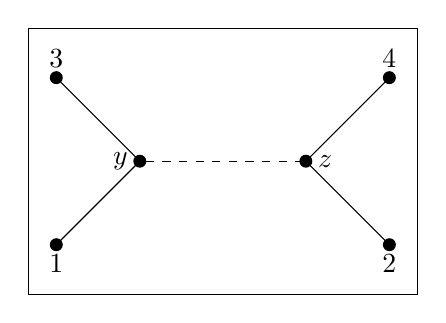
\begin{tikzpicture}[framed, baseline={(current bounding box.center)}]
%Dia1
              \begin{feynman}
                \vertex [dot] (a) {} ;
                \vertex [right = 6em of a, dot] (b) {} ;
                \vertex [above left=of a, dot]  (i1) {};
                \vertex [below left =of a, dot] (i2) {};
                \vertex [above right=of b, dot] (i3) {};
                \vertex [below right=of b, dot] (i4) {};
                \diagram * {
                  (i1) -- [plain] (a),
                  (i2) -- [plain] (a),
                  (i3) -- [plain] (b),
                  (i4) -- [plain] (b),
                  (a) -- [dashed] (b),
                };
                \vertex [left = 0.7em of a] {$y$};
                \vertex [right = 0.7em of b] {$z$};
                \vertex [above= 0.7em of i1] {$3$};
                \vertex [below= 0.7em of i2] {$1$};
                \vertex [above = 0.7em of i3] {$4$};
                \vertex [below = 0.7em of i4] {$2$};
              \end{feynman}
            \end{tikzpicture}
          }
          \resizebox{.4\textwidth}{.1\textwidth}{
%Dia2
            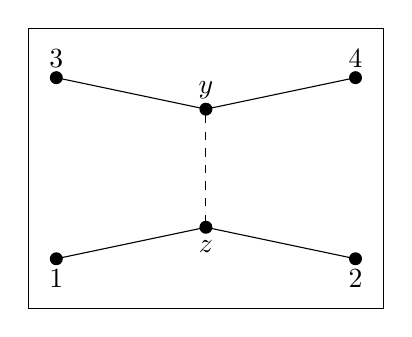
\begin{tikzpicture}[framed, baseline={(current bounding box.center)}]
              \begin{feynman}
                \vertex [dot] at (0,0) (a) {} ;
                \vertex [dot] at (0, -1.5) (b) {} ;
                \vertex [dot] at (-1.9, 0.4)  (i1) {};
                \vertex [dot] at (-1.9, -1.9) (i2) {};
                \vertex [dot] at (1.9, 0.4) (i3) {};
                \vertex [dot] at (1.9, -1.9) (i4) {};
                \diagram * {
                  (i1) -- [plain] (a),
                  (i2) -- [plain] (b),
                  (i3) -- [plain] (a),
                  (i4) -- [plain] (b),
                  (a) -- [dashed] (b),
                };
                \vertex [above= 0.7em of a] {$y$};
                \vertex [below= 0.7em of b] {$z$};
                \vertex [above= 0.7em of i1] {$3$};
                \vertex [below= 0.7em of i2] {$1$};
                \vertex [above = 0.7em of i3] {$4$};
                \vertex [below = 0.7em of i4] {$2$};
              \end{feynman}
            \end{tikzpicture}
          }
          \resizebox{.4\textwidth}{.1\textwidth}{
            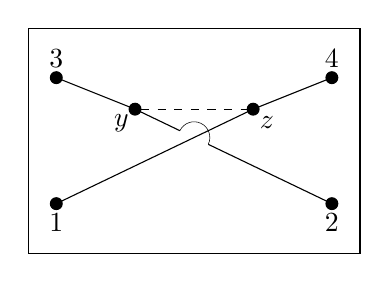
\begin{tikzpicture}[framed, baseline={(current bounding box.center)}]
%Dia3
              \begin{feynman}
                \vertex [dot] at (0,0) (a) {} ;
                \vertex [dot] at (1.5,0) (b) {} ;
                \vertex [dot] at (-1, 0.4) (i1) {};
                \vertex [dot] at (-1, -1.2) (i2) {};
                \vertex [dot] at (2.5, 0.4) (i3) {};
                \vertex [dot] at (2.5, -1.2) (i4) {};
                \diagram * {
                  (i1) -- [plain] (a),
                  (i2) -- [plain] (b),
                  (i3) -- [plain] (b),
%                  (i4) -- [plain] (a),
                  (a) -- [dashed] (b),
                };
                \vertex [below left = 0.7em of a] {$y$};
                \vertex [below right = 0.7em of b] {$z$};
                \vertex [above= 0.7em of i1] {$3$};
                \vertex [below= 0.7em of i2] {$1$};
                \vertex [above = 0.7em of i3] {$4$};
                \vertex [below = 0.7em of i4] {$2$};

                \path [name path=line 1] (i2) -- (b);
                \path [name path=line 2] (i4) -- (a);
                \path [name intersections={of = line 1 and line 2}];
                \coordinate (S)  at (intersection-1);
                \path[name path=circle] (S) circle(0.2);
                \path [name intersections={of = circle and line 2}];
                \coordinate (K1)  at (intersection-1);
                \coordinate (K2)  at (intersection-2);
                \draw (i4) -- (K2);
                \draw (K1) -- (a);
                \tkzDrawArc[color=black](S,K2)(K1);
              \end{feynman}
            \end{tikzpicture}
          }
            \end{center}
            \begin{center}
              \resizebox{.4\textwidth}{.1\textwidth}{
              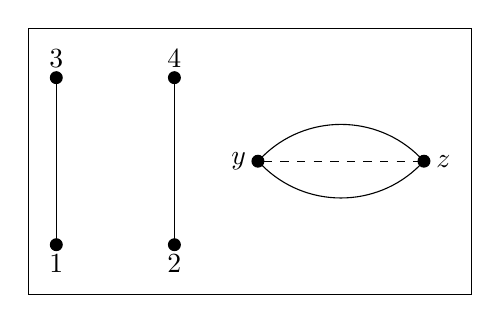
\begin{tikzpicture}[framed, baseline={(current bounding box.center)}]
%Dia4
                \begin{feynman}
                  \vertex [dot] (a) {} ;
                  \vertex [right = 6em of a, dot] (b) {} ;
                  \vertex [above left=of a, dot] (i1) {};
                  \vertex [below left =of a, dot] (i2) {};
                  \vertex [left=of i1,dot] (i3) {};
                  \vertex [left=of i2,dot] (i4) {};
                  \diagram * {
                    (i1) -- [plain] (i2),
                    (i3) -- [plain] (i4),
                    (a) -- [dashed] (b),
                    (a) -- [out=45, in=135, min distance=0.5cm] (b) -- [out=225, in=-45, min distance=0.5cm] (a),
                  };
                  \vertex [left = 0.7em of a] {$y$};
                  \vertex [right = 0.7em of b] {$z$};
                  \vertex [above= 0.7em of i1] {$4$};
                  \vertex [below= 0.7em of i2] {$2$};
                  \vertex [above = 0.7em of i3] {$3$};
                  \vertex [below = 0.7em of i4] {$1$};
                \end{feynman}
              \end{tikzpicture} 
            }
%            $\qquad$
            \resizebox{.4\textwidth}{.1\textwidth}{
            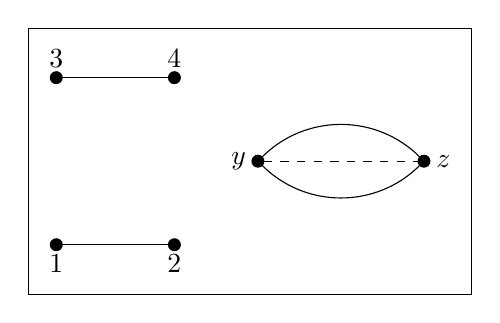
\begin{tikzpicture}[framed, baseline={(current bounding box.center)}]
%Dia5
              \begin{feynman}
                \vertex [dot] (a) {} ;
                \vertex [right = 6em of a, dot] (b) {} ;
                \vertex [above left=of a, dot] (i1) {};
                \vertex [below left =of a, dot] (i2) {};
                \vertex [left=of i1,dot] (i3) {};
                \vertex [left=of i2,dot] (i4) {};
                \diagram * {
                  (i1) -- [plain] (i3),
                  (i2) -- [plain] (i4),
                  (a) -- [dashed] (b),
                  (a) -- [out=45, in=135, min distance=0.5cm] (b) -- [out=225, in=-45, min distance=0.5cm] (a),
                };
                \vertex [left = 0.7em of a] {$y$};
                \vertex [right = 0.7em of b] {$z$};
                \vertex [above= 0.7em of i1] {$4$};
                \vertex [below= 0.7em of i2] {$2$};
                \vertex [above = 0.7em of i3] {$3$};
                \vertex [below = 0.7em of i4] {$1$};
              \end{feynman}
            \end{tikzpicture}
          }
            \resizebox{.4\textwidth}{.1\textwidth}{
            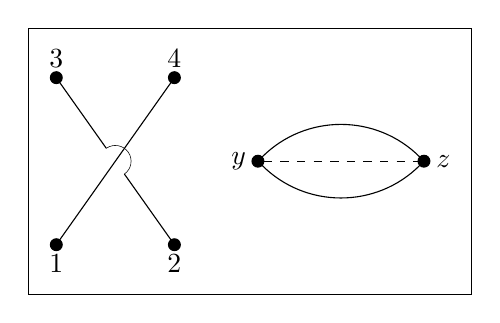
\begin{tikzpicture}[framed, baseline={(current bounding box.center)}]
%Dia6
              \begin{feynman}
                \vertex [dot] (a) {} ;
                \vertex [right = 6em of a, dot] (b) {} ;
                \vertex [above left=of a, dot] (i1) {};
                \vertex [below left =of a, dot] (i2) {};
                \vertex [left=of i1,dot] (i3) {};
                \vertex [left=of i2,dot] (i4) {};
                \diagram * {
                  (i1) -- [plain] (i4),
                  %(i2) -- [plain] (i3),
                  (a) -- [dashed] (b),
                  (a) -- [out=45, in=135, min distance=0.5cm] (b) -- [out=225, in=-45, min distance=0.5cm] (a),
                };
                \path [name path=line 1] (i1) -- (i4);
                \path [name path=line 2] (i2) -- (i3);
                \path [name intersections={of = line 1 and line 2}];
                \coordinate (S)  at (intersection-1);
                \path[name path=circle] (S) circle(0.2);
                \path [name intersections={of = circle and line 2}];
                \coordinate (K1)  at (intersection-1);
                \coordinate (K2)  at (intersection-2);
                \draw (i2) -- (K2);
                \draw (K1) -- (i3);
                \tkzDrawArc[color=black](S,K2)(K1);
                \vertex [left = 0.7em of a] {$y$};
                \vertex [right = 0.7em of b] {$z$};
                \vertex [above= 0.7em of i1] {$4$};
                \vertex [below= 0.7em of i2] {$2$};
                \vertex [above = 0.7em of i3] {$3$};
                \vertex [below = 0.7em of i4] {$1$};
              \end{feynman}
            \end{tikzpicture} %$\qquad$ 
          }
            \resizebox{.4\textwidth}{.1\textwidth}{
              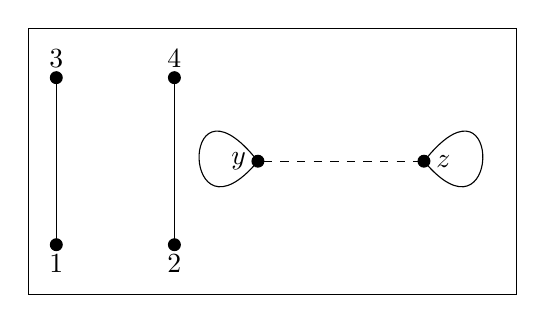
\begin{tikzpicture}[framed, baseline={(current bounding box.center)}]
%Dia7
                \begin{feynman}
                  \vertex [dot] (a) {} ;
                  \vertex [right = 6em of a, dot] (b) {} ;
                  \vertex [above left=of a, dot] (i1) {};
                  \vertex [below left =of a, dot] (i2) {};
                  \vertex [left=of i1,dot] (i3) {};
                  \vertex [left=of i2,dot] (i4) {};
                  \vertex (q) at (a);
                  \vertex (r) at (b);
                  \diagram * {
                    (i1) -- [plain] (i2),
                    (i3) -- [plain] (i4),
                    (a) -- [dashed] (b),
                    (a) -- [out=130, in=230, loop, min distance=1.5cm] (q),
%                    (a) -- [loop] node [left] {} (a),
                    (b) -- [out=50, in=-50, loop, min distance=1.5cm] (r),
                  };
                  \vertex [left = 0.7em of a] {$y$};
                  \vertex [right = 0.7em of b] {$z$};
                  \vertex [above= 0.7em of i1] {$4$};
                  \vertex [below= 0.7em of i2] {$2$};
                  \vertex [above = 0.7em of i3] {$3$};
                  \vertex [below = 0.7em of i4] {$1$};
                \end{feynman}
              \end{tikzpicture} %$\qquad$
            }
            \resizebox{.4\textwidth}{.1\textwidth}{
            \begin{tikzpicture}[framed, baseline={(current bounding box.center)}]
%Dia8
              \begin{feynman}
                \vertex [dot] (a) {} ;
                \vertex [right = 6em of a, dot] (b) {} ;
                \vertex [above left=of a, dot] (i1) {};
                \vertex [below left =of a, dot] (i2) {};
                \vertex [left=of i1,dot] (i3) {};
                \vertex [left=of i2,dot] (i4) {};
                \diagram * {
                  (i1) -- [plain] (i3),
                  (i2) -- [plain] (i4),
                  (a) -- [dashed] (b),
                  (a) -- [out=130, in=230, loop, min distance=1.5cm] (q),
%                    (a) -- [loop] node [left] {} (a),
                  (b) -- [out=50, in=-50, loop, min distance=1.5cm] (r),
                };
                \vertex [left = 0.7em of a] {$y$};
                \vertex [right = 0.7em of b] {$z$};
                \vertex [above= 0.7em of i1] {$4$};
                \vertex [below= 0.7em of i2] {$2$};
                \vertex [above = 0.7em of i3] {$3$};
                \vertex [below = 0.7em of i4] {$1$};
              \end{feynman}
            \end{tikzpicture} %$\qquad$
          }
            \resizebox{.4\textwidth}{.1\textwidth}{
            \begin{tikzpicture}[framed, baseline={(current bounding box.center)}]
%Dia9
              \begin{feynman}
                \vertex [dot] (a) {} ;
                \vertex [right = 6em of a, dot] (b) {} ;
                \vertex [above left=of a, dot] (i1) {};
                \vertex [below left =of a, dot] (i2) {};
                \vertex [left=of i1,dot] (i3) {};
                \vertex [left=of i2,dot] (i4) {};
                \diagram * {
                  (i1) -- [plain] (i4),
                  %(i2) -- [plain] (i3),
                  (a) -- [dashed] (b),
                  (a) -- [out=130, in=230, loop, min distance=1.5cm] (q),
%                    (a) -- [loop] node [left] {} (a),
                  (b) -- [out=50, in=-50, loop, min distance=1.5cm] (r),
                };
                \path [name path=line 1] (i1) -- (i4);
                \path [name path=line 2] (i2) -- (i3);
                \path [name intersections={of = line 1 and line 2}];
                \coordinate (S)  at (intersection-1);
                \path[name path=circle] (S) circle(0.2);
                \path [name intersections={of = circle and line 2}];
                \coordinate (K1)  at (intersection-1);
                \coordinate (K2)  at (intersection-2);
                \draw (i2) -- (K2);
                \draw (K1) -- (i3);
                \tkzDrawArc[color=black](S,K2)(K1);
                \vertex [left = 0.7em of a] {$y$};
                \vertex [right = 0.7em of b] {$z$};
                \vertex [above= 0.7em of i1] {$4$};
                \vertex [below= 0.7em of i2] {$2$};
                \vertex [above = 0.7em of i3] {$3$};
                \vertex [below = 0.7em of i4] {$1$};
              \end{feynman}
            \end{tikzpicture} }
            \resizebox{.4\textwidth}{.1\textwidth}{
            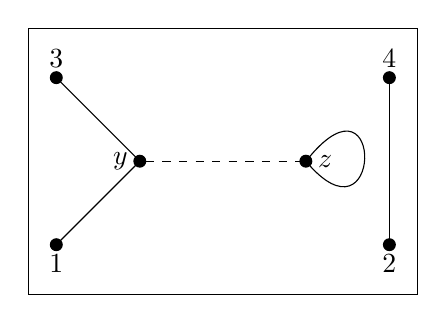
\begin{tikzpicture}[framed, baseline={(current bounding box.center)}]
%Dia10
                \begin{feynman}
                  \vertex [dot] (a) {} ;
                  \vertex [right = 6em of a, dot] (b) {} ;
                  \vertex [above left=of a, dot] (i1) {};
                  \vertex [below left =of a, dot] (i2) {};
                  \vertex [above right=of b,dot] (i3) {};
                  \vertex [below right=of b,dot] (i4) {};
                  \vertex (q) at (a);
                  \vertex (r) at (b);
                  \diagram * {
                    (i3) -- [plain] (i4),
                    (a) -- [dashed] (b),
                    (a)-- [plain] (i1),
                    (a)-- [plain] (i2),
%                    (a) -- [loop] node [left] {} (a),
                    (b) -- [out=50, in=-50, loop, min distance=1.5cm] (r),
                  };
                  \vertex [left = 0.7em of a] {$y$};
                  \vertex [right = 0.7em of b] {$z$};
                  \vertex [above= 0.7em of i1] {$3$};
                  \vertex [below= 0.7em of i2] {$1$};
                  \vertex [above = 0.7em of i3] {$4$};
                  \vertex [below = 0.7em of i4] {$2$};
                \end{feynman}
            \end{tikzpicture} }%$\qquad$
            \resizebox{.4\textwidth}{.1\textwidth}{
            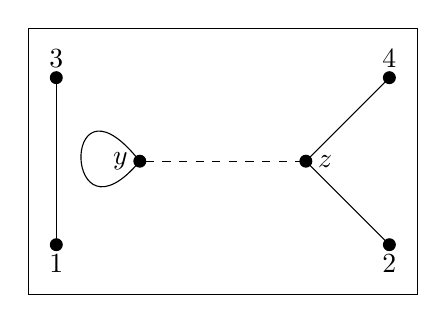
\begin{tikzpicture}[framed, baseline={(current bounding box.center)}]
%Dia11
                \begin{feynman}
                  \vertex [dot] (a) {} ;
                  \vertex [right = 6em of a, dot] (b) {} ;
                  \vertex [above left=of a, dot] (i1) {};
                  \vertex [below left =of a, dot] (i2) {};
                  \vertex [above right=of b,dot] (i3) {};
                  \vertex [below right=of b,dot] (i4) {};
                  \vertex (q) at (a);
                  \vertex (r) at (b);
                  \diagram * {
                    (i3) -- [plain] (b) -- [plain] (i4),
                    (a) -- [dashed] (b),
                    (i1)-- [plain] (i2),
%                    (a) -- [loop] node [left] {} (a),
                  (a) -- [out=130, in=230, loop, min distance=1.5cm] (q),
%                    (b) -- [out=50, in=-50, loop, min distance=1.5cm] (r),
                  };
                  \vertex [left = 0.7em of a] {$y$};
                  \vertex [right = 0.7em of b] {$z$};
                  \vertex [above= 0.7em of i1] {$3$};
                  \vertex [below= 0.7em of i2] {$1$};
                  \vertex [above = 0.7em of i3] {$4$};
                  \vertex [below = 0.7em of i4] {$2$};
                \end{feynman}
            \end{tikzpicture} }%$\qquad$

            \resizebox{.4\textwidth}{.1\textwidth}{
            \begin{tikzpicture}[framed, baseline={(current bounding box.center)}]
%Dia12
              \begin{feynman}
                \vertex [dot] (a) {} ;
                \vertex [right = 6em of a, dot] (b) {} ;
                \vertex [above left=of a, dot] (i1) {};
                \vertex [below left =of a, dot] (i2) {};
                \vertex [left=of i1,dot] (i3) {};
                \vertex [left=of i2,dot] (i4) {};
                \diagram * {
                  (i1) -- [plain] (i3),
                  (i2) -- [plain] (a) -- [plain] (i4),
                  (a) -- [dashed] (b),
%                  (a) -- [out=130, in=230, loop, min distance=1.5cm] (q),
%                    (a) -- [loop] node [left] {} (a),
                  (b) -- [out=50, in=-50, loop, min distance=1.5cm] (r),
                };
                \vertex [left = 0.7em of a] {$y$};
                \vertex [right = 0.7em of b] {$z$};
                \vertex [above= 0.7em of i1] {$4$};
                \vertex [below= 0.7em of i2] {$2$};
                \vertex [above = 0.7em of i3] {$3$};
                \vertex [below = 0.7em of i4] {$1$};
              \end{feynman}
            \end{tikzpicture} }%$\qquad$
            \resizebox{.4\textwidth}{.1\textwidth}{
            \begin{tikzpicture}[framed, baseline={(current bounding box.center)}]
%Dia13
              \begin{feynman}
                \vertex [dot] (a) {} ;
                \vertex [right = 6em of a, dot] (b) {} ;
                \vertex [above left=of a, dot] (i1) {};
                \vertex [below left =of a, dot] (i2) {};
                \vertex [left=of i1,dot] (i3) {};
                \vertex [left=of i2,dot] (i4) {};
                \diagram * {
                  (i4) -- [plain] (i2),
                  (i1) -- [plain] (a) -- [plain] (i3),
                  (a) -- [dashed] (b),
%                  (a) -- [out=130, in=230, loop, min distance=1.5cm] (q),
%                    (a) -- [loop] node [left] {} (a),
                  (b) -- [out=50, in=-50, loop, min distance=1.5cm] (r),
                };
                \vertex [left = 0.7em of a] {$y$};
                \vertex [right = 0.7em of b] {$z$};
                \vertex [above= 0.7em of i1] {$4$};
                \vertex [below= 0.7em of i2] {$2$};
                \vertex [above = 0.7em of i3] {$3$};
                \vertex [below = 0.7em of i4] {$1$};
              \end{feynman}
            \end{tikzpicture} }
          %$\qquad$

            \resizebox{.4\textwidth}{.1\textwidth}{
            \begin{tikzpicture}[framed, baseline={(current bounding box.center)}]
%Dia14
              \begin{feynman}
                \vertex [dot] (a) {} ;
                \vertex [right = 6em of a, dot] (b) {} ;
                \vertex [above left=of a, dot] (i1) {};
                \vertex [below left =of a, dot] (i2) {};
                \vertex [left=of i1,dot] (i3) {};
                \vertex [left=of i2,dot] (i4) {};
                \diagram * {
                  %(i1) -- [plain] (i4),
                  %(i2) -- [plain] (i3),
                  (a) -- [dashed] (b),
                  (i1) -- [plain] (a) -- [plain] (i4);
%                  (a) -- [out=130, in=230, loop, min distance=1.5cm] (q),
%                    (a) -- [loop] node [left] {} (a),
                  (b) -- [out=50, in=-50, loop, min distance=1.5cm] (r),
                };
                \path [name path=line 1] (a) -- (i4);
                \path [name path=line 2] (i2) -- (i3);
                \path [name intersections={of = line 1 and line 2}];
                \coordinate (S)  at (intersection-1);
                \path[name path=circle] (S) circle(0.2);
                \path [name intersections={of = circle and line 2}];
                \coordinate (K1)  at (intersection-1);
                \coordinate (K2)  at (intersection-2);
                \draw (i2) -- (K2);
                \draw (K1) -- (i3);
                \tkzDrawArc[color=black](S,K2)(K1);
                \vertex [left = 0.7em of a] {$y$};
                \vertex [right = 0.7em of b] {$z$};
                \vertex [above= 0.7em of i1] {$4$};
                \vertex [below= 0.7em of i2] {$2$};
                \vertex [above = 0.7em of i3] {$3$};
                \vertex [below = 0.7em of i4] {$1$};
              \end{feynman}
            \end{tikzpicture} %$\qquad $
          }
            \resizebox{.4\textwidth}{.1\textwidth}{
            \begin{tikzpicture}[framed, baseline={(current bounding box.center)}]
%Dia15
              \begin{feynman}
                \vertex [dot] (a) {} ;
                \vertex [right = 6em of a, dot] (b) {} ;
                \vertex [above left=of a, dot] (i1) {};
                \vertex [below left =of a, dot] (i2) {};
                \vertex [left=of i1,dot] (i3) {};
                \vertex [left=of i2,dot] (i4) {};
                \diagram * {
                  (i1) -- [plain] (i4),
                  (i2) -- [plain] (a),
                  %(i2) -- [plain] (i3),
                  (a) -- [dashed] (b),
%                  (a) -- [out=130, in=230, loop, min distance=1.5cm] (q),
%                    (a) -- [loop] node [left] {} (a),
                  (b) -- [out=50, in=-50, loop, min distance=1.5cm] (r),
                };
                \path [name path=line 1] (i1) -- (i4);
                \path [name path=line 2] (i3) -- (a);
                \path [name intersections={of = line 1 and line 2}];
                \coordinate (S)  at (intersection-1);
                \path[name path=circle] (S) circle(0.2);
                \path [name intersections={of = circle and line 2}];
                \coordinate (K1)  at (intersection-1);
                \coordinate (K2)  at (intersection-2);
                \draw (a) -- (K2);
                \draw (K1) -- (i3);
                \tkzDrawArc[color=black](S,K2)(K1);
                \vertex [left = 0.7em of a] {$y$};
                \vertex [right = 0.7em of b] {$z$};
                \vertex [above= 0.7em of i1] {$4$};
                \vertex [below= 0.7em of i2] {$2$};
                \vertex [above = 0.7em of i3] {$3$};
                \vertex [below = 0.7em of i4] {$1$};
              \end{feynman}
            \end{tikzpicture}% \\ 
          }

            \resizebox{.4\textwidth}{.1\textwidth}{
            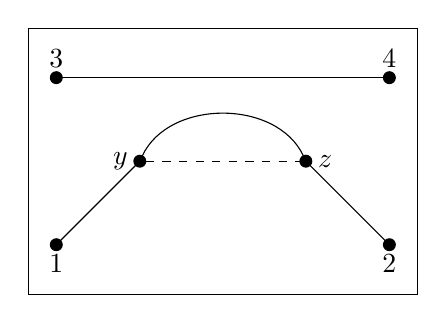
\begin{tikzpicture}[framed, baseline={(current bounding box.center)}]
%Dia16
              \begin{feynman}
                \vertex [dot] (a) {} ;
                \vertex [right = 6em of a, dot] (b) {} ;
                \vertex [above left=of a, dot]  (i1) {};
                \vertex [below left =of a, dot] (i2) {};
                \vertex [above right=of b, dot] (i3) {};
                \vertex [below right=of b, dot] (i4) {};
                \diagram * {
                  (i1) -- [plain] (i3),
                  (i2) -- [plain] (a),
%                  (i3) -- [plain] (b),
                  (i4) -- [plain] (b),
                  (a) -- [dashed] (b),
                  (a) -- [out=65, in=115, min distance=0.5cm] (b),% -- [out=225, in=-45, min distance=0.5cm] (a),
                };
                \vertex [left = 0.7em of a] {$y$};
                \vertex [right = 0.7em of b] {$z$};
                \vertex [above= 0.7em of i1] {$3$};
                \vertex [below= 0.7em of i2] {$1$};
                \vertex [above = 0.7em of i3] {$4$};
                \vertex [below = 0.7em of i4] {$2$};
              \end{feynman}
            \end{tikzpicture} }%$\qquad \phantom{=} \quad$
%Dia17
            \resizebox{.4\textwidth}{.1\textwidth}{
            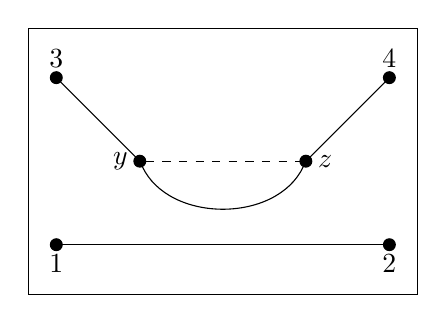
\begin{tikzpicture}[framed, baseline={(current bounding box.center)}]
              \begin{feynman}
                \vertex [dot] (a) {} ;
                \vertex [right = 6em of a, dot] (b) {} ;
                \vertex [above left=of a, dot]  (i1) {};
                \vertex [below left =of a, dot] (i2) {};
                \vertex [above right=of b, dot] (i3) {};
                \vertex [below right=of b, dot] (i4) {};
                \diagram * {
                  (i2) -- [plain] (i4),
                  (i1) -- [plain] (a),
%                  (i3) -- [plain] (b),
                  (i3) -- [plain] (b),
                  (a) -- [dashed] (b),
                  (a) -- [out=-65, in=-115, min distance=0.5cm] (b),% -- [out=225, in=-45, min distance=0.5cm] (a),
                };
                \vertex [left = 0.7em of a] {$y$};
                \vertex [right = 0.7em of b] {$z$};
                \vertex [above= 0.7em of i1] {$3$};
                \vertex [below= 0.7em of i2] {$1$};
                \vertex [above = 0.7em of i3] {$4$};
                \vertex [below = 0.7em of i4] {$2$};
              \end{feynman}
            \end{tikzpicture}}
%Dia18
            \resizebox{.4\textwidth}{.1\textwidth}{
            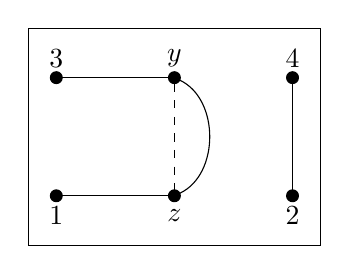
\begin{tikzpicture}[framed, baseline={(current bounding box.center)}]
              \begin{feynman}
                \vertex [dot] (a) {} ;
                \vertex [below = of a, dot] (b) {} ;
                \vertex [left=of a, dot]  (i1) {};
                \vertex [left =of b, dot] (i2) {};
                \vertex [right=of a, dot] (i3) {};
                \vertex [right=of b, dot] (i4) {};
                \diagram * {
                  (i4) -- [plain] (i3),
                  (a) -- [plain] (i1),
%                  (i3) -- [plain] (b),
                  (i2) -- [plain] (b),
                  (a) -- [dashed] (b),
                  (a) -- [out=-25, in=25, min distance=0.5cm] (b),% -- [out=225, in=-45, min distance=0.5cm] (a),
                };
                \vertex [above = 0.7em of a] {$y$};
                \vertex [below = 0.7em of b] {$z$};
                \vertex [above= 0.7em of i1] {$3$};
                \vertex [below= 0.7em of i2] {$1$};
                \vertex [above = 0.7em of i3] {$4$};
                \vertex [below = 0.7em of i4] {$2$};
              \end{feynman}
            \end{tikzpicture}
          }
%Dia19
            %$\qquad \phantom{=} \quad$
            \resizebox{.4\textwidth}{.1\textwidth}{
            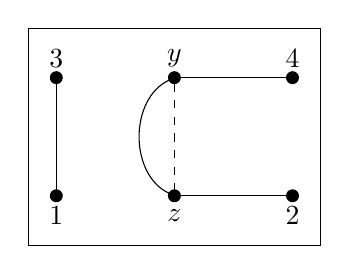
\begin{tikzpicture}[framed, baseline={(current bounding box.center)}]
              \begin{feynman}
                \vertex [dot] (a) {} ;
                \vertex [below = of a, dot] (b) {} ;
                \vertex [left=of a, dot]  (i1) {};
                \vertex [left =of b, dot] (i2) {};
                \vertex [right=of a, dot] (i3) {};
                \vertex [right=of b, dot] (i4) {};
                \diagram * {
                  (a) -- [plain] (i3),
                  (i1) -- [plain] (i2),
%                  (i3) -- [plain] (b),
                  (i4) -- [plain] (b),
                  (a) -- [dashed] (b),
                  (a) -- [out=-155, in=155, min distance=0.5cm] (b),% -- [out=225, in=-45, min distance=0.5cm] (a),
                };
                \vertex [above = 0.7em of a] {$y$};
                \vertex [below = 0.7em of b] {$z$};
                \vertex [above= 0.7em of i1] {$3$};
                \vertex [below= 0.7em of i2] {$1$};
                \vertex [above = 0.7em of i3] {$4$};
                \vertex [below = 0.7em of i4] {$2$};
              \end{feynman}
            \end{tikzpicture}
          }
%Dia20
            \resizebox{.4\textwidth}{.1\textwidth}{
            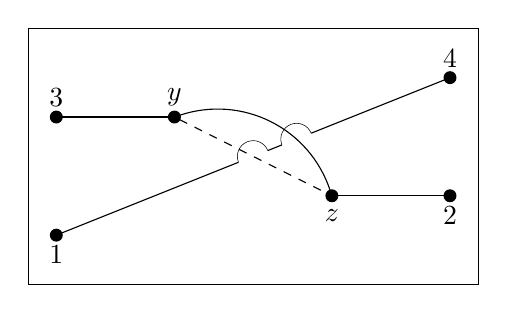
\begin{tikzpicture}[framed, baseline={(current bounding box.center)}]
              \begin{feynman}
                \vertex [dot] at (0,0) (a) {} ;
                \vertex [dot] at (2, -1) (b) {} ;
                \vertex [left=of a, dot]  (i1) {};
                \vertex [below=of i1, dot] (i2) {};
                \vertex [right=of b, dot] (i4) {};
                \vertex [above=of i4, dot] (i3) {};
                \diagram * {
%                  (i2) -- [plain] (i3),
                  (a) -- [plain] (i1),
%                  (i3) -- [plain] (b),
                  (i4) -- [plain] (b),
%                  (a) -- [dashed] (b),
                  (a) -- [out=18.4349, in=108.4349, min distance=0.5cm] (b),% -- [out=225, in=-45, min distance=0.5cm] (a),
                };
                \vertex [above = 0.7em of a] {$y$};
                \vertex [below = 0.7em of b] {$z$};
                \vertex [above= 0.7em of i1] {$3$};
                \vertex [below= 0.7em of i2] {$1$};
                \vertex [above = 0.7em of i3] {$4$};
                \vertex [below = 0.7em of i4] {$2$};

                \draw[dashed, name path=line 1] (a) -- (b);
                \path [name path=line 2] (i3) -- (i2);
                \path [name path=line 3] (a) to[out=18.4349, in=108.4349, min distance=0.5cm] (b);
                \path [name intersections={of = line 1 and line 2}];
                \coordinate (S)  at (intersection-1);
                \path[name path=circle] (S) circle(0.2);
                \path [name intersections={of = circle and line 2}];
                \coordinate (K1)  at (intersection-1);
                \coordinate (K2)  at (intersection-2);
                \tkzDrawArc[color=black](S,K1)(K2);

                \path [name intersections={of = line 2 and line 3}];
                \coordinate (S2)  at (intersection-1);
                \path[name path=circle] (S2) circle(0.2);
                \path [name intersections={of = circle and line 2}];
                \coordinate (K3)  at (intersection-1);
                \coordinate (K4)  at (intersection-2);

                \tkzDrawArc[color=black](S2,K3)(K4);
                \draw (i3) -- (K3);
                \draw (K4) -- (K1);
                \draw (K2) -- (i2);
              \end{feynman}
            \end{tikzpicture}
          }
%Dia21
            %$\qquad \phantom{=} \quad$
            \resizebox{.4\textwidth}{.1\textwidth}{
            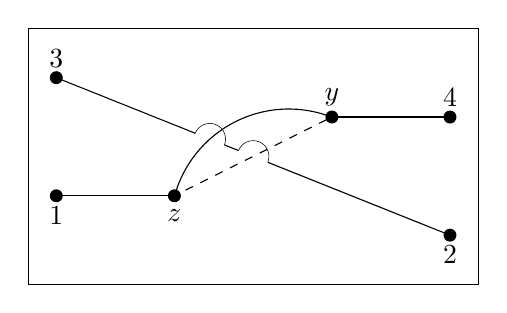
\begin{tikzpicture}[framed, baseline={(current bounding box.center)}]
              \begin{feynman}
                \vertex [dot] at (0,0) (a) {} ;
                \vertex [dot] at (-2,-1) (b) {} ;
                \vertex [left =of b, dot] (i2) {};
                \vertex [above=of i2, dot]  (i1) {};
                \vertex [right=of a, dot] (i3) {};
                \vertex [below=of i3, dot] (i4) {};
%                \draw[] (b) to[out=71.565, in=161.565, min distance=0.5cm] (i1);%[out=71.565, in=161.565, min distance=0.5cm] (c);% -- [out=225, in=-45, min distance=0.5cm] (a),
                \diagram * {
                  (a) -- [plain] (i3),
%                  (i1) -- [plain] (i4),
%                  (i3) -- [plain] (b),
                  (i2) -- [plain] (b),
%                  (a) -- [dashed] (b),
                  (b) -- [out=71.565, in=161.565, min distance=0.5cm] (a),% -- [out=225, in=-45, min distance=0.5cm] (a),
                };
                \vertex [above = 0.7em of a] {$y$};
                \vertex [below = 0.7em of b] {$z$};
                \vertex [above= 0.7em of i1] {$3$};
                \vertex [below= 0.7em of i2] {$1$};
                \vertex [above = 0.7em of i3] {$4$};
                \vertex [below = 0.7em of i4] {$2$};

                \draw[dashed, name path=line 1] (a) -- (b);
                \path [name path=line 2] (i4) -- (i1);
                \path [name path=line 3] (b) to[out=71.565, in=161.565, min distance=0.5cm] (a);
                \path [name intersections={of = line 1 and line 2}];
                \coordinate (S)  at (intersection-1);
                \path[name path=circle] (S) circle(0.2);
                \path [name intersections={of = circle and line 2}];
                \coordinate (K1)  at (intersection-1);
                \coordinate (K2)  at (intersection-2);
                \tkzDrawArc[color=black](S,K2)(K1);

                \path [name intersections={of = line 2 and line 3}];
                \coordinate (S2)  at (intersection-1);
                \path[name path=circle] (S2) circle(0.2);
                \path [name intersections={of = circle and line 2}];
                \coordinate (K3)  at (intersection-1);
                \coordinate (K4)  at (intersection-2);

                \tkzDrawArc[color=black](S2,K4)(K3);
                \draw (i1) -- (K3);
                \draw (K4) -- (K1);
                \draw (K2) -- (i4);
              \end{feynman}
            \end{tikzpicture}
          }%\\
            \end{center}
          \item
            Here are the diagrams:
            \begin{center}
              \resizebox{.4\textwidth}{.1\textwidth}{
            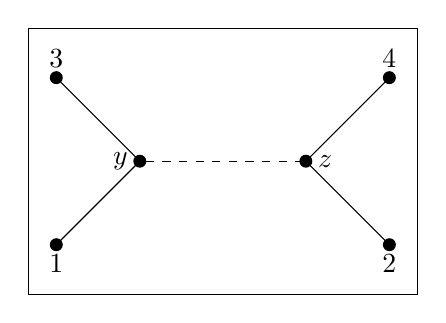
\begin{tikzpicture}[framed, baseline={(current bounding box.center)}]
              \begin{feynman}
                \vertex [dot] (a) {} ;
                \vertex [right = 6em of a, dot] (b) {} ;
                \vertex [above left=of a, dot]  (i1) {};
                \vertex [below left =of a, dot] (i2) {};
                \vertex [above right=of b, dot] (i3) {};
                \vertex [below right=of b, dot] (i4) {};
                \diagram * {
                  (i1) -- [plain] (a),
                  (i2) -- [plain] (a),
                  (i3) -- [plain] (b),
                  (i4) -- [plain] (b),
                  (a) -- [dashed] (b),
                };
                \vertex [left = 0.7em of a] {$y$};
                \vertex [right = 0.7em of b] {$z$};
                \vertex [above= 0.7em of i1] {$3$};
                \vertex [below= 0.7em of i2] {$1$};
                \vertex [above = 0.7em of i3] {$4$};
                \vertex [below = 0.7em of i4] {$2$};
              \end{feynman}
            \end{tikzpicture}
          }
          \resizebox{.4\textwidth}{.1\textwidth}{
            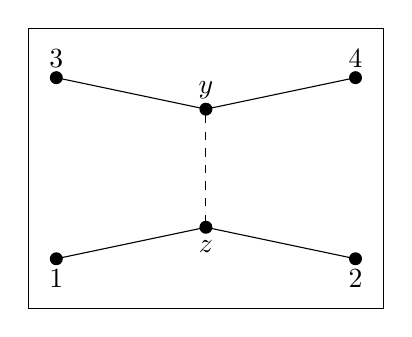
\begin{tikzpicture}[framed, baseline={(current bounding box.center)}]
              \begin{feynman}
                \vertex [dot] at (0,0) (a) {} ;
                \vertex [dot] at (0, -1.5) (b) {} ;
                \vertex [dot] at (-1.9, 0.4)  (i1) {};
                \vertex [dot] at (-1.9, -1.9) (i2) {};
                \vertex [dot] at (1.9, 0.4) (i3) {};
                \vertex [dot] at (1.9, -1.9) (i4) {};
                \diagram * {
                  (i1) -- [plain] (a),
                  (i2) -- [plain] (b),
                  (i3) -- [plain] (a),
                  (i4) -- [plain] (b),
                  (a) -- [dashed] (b),
                };
                \vertex [above= 0.7em of a] {$y$};
                \vertex [below= 0.7em of b] {$z$};
                \vertex [above= 0.7em of i1] {$3$};
                \vertex [below= 0.7em of i2] {$1$};
                \vertex [above = 0.7em of i3] {$4$};
                \vertex [below = 0.7em of i4] {$2$};
              \end{feynman}
            \end{tikzpicture}
          }
          \resizebox{.4\textwidth}{.1\textwidth}{
            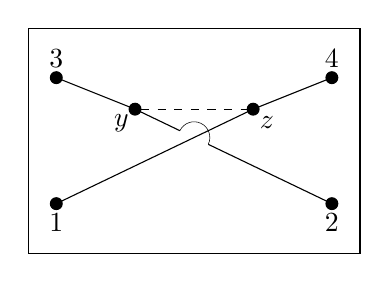
\begin{tikzpicture}[framed, baseline={(current bounding box.center)}]
              \begin{feynman}
                \vertex [dot] at (0,0) (a) {} ;
                \vertex [dot] at (1.5,0) (b) {} ;
                \vertex [dot] at (-1, 0.4) (i1) {};
                \vertex [dot] at (-1, -1.2) (i2) {};
                \vertex [dot] at (2.5, 0.4) (i3) {};
                \vertex [dot] at (2.5, -1.2) (i4) {};
                \diagram * {
                  (i1) -- [plain] (a),
                  (i2) -- [plain] (b),
                  (i3) -- [plain] (b),
%                  (i4) -- [plain] (a),
                  (a) -- [dashed] (b),
                };
                \vertex [below left = 0.7em of a] {$y$};
                \vertex [below right = 0.7em of b] {$z$};
                \vertex [above= 0.7em of i1] {$3$};
                \vertex [below= 0.7em of i2] {$1$};
                \vertex [above = 0.7em of i3] {$4$};
                \vertex [below = 0.7em of i4] {$2$};

                \path [name path=line 1] (i2) -- (b);
                \path [name path=line 2] (i4) -- (a);
                \path [name intersections={of = line 1 and line 2}];
                \coordinate (S)  at (intersection-1);
                \path[name path=circle] (S) circle(0.2);
                \path [name intersections={of = circle and line 2}];
                \coordinate (K1)  at (intersection-1);
                \coordinate (K2)  at (intersection-2);
                \draw (i4) -- (K2);
                \draw (K1) -- (a);
                \tkzDrawArc[color=black](S,K2)(K1);
              \end{feynman}
            \end{tikzpicture}
          }
            \end{center}
            \begin{center}
            \resizebox{.4\textwidth}{.1\textwidth}{
            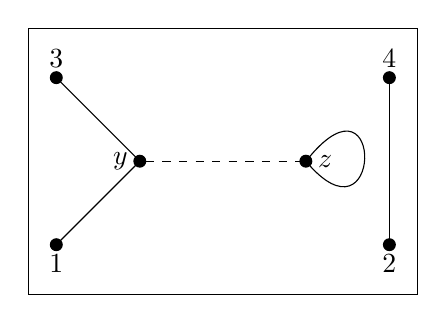
\begin{tikzpicture}[framed, baseline={(current bounding box.center)}]
                \begin{feynman}
                  \vertex [dot] (a) {} ;
                  \vertex [right = 6em of a, dot] (b) {} ;
                  \vertex [above left=of a, dot] (i1) {};
                  \vertex [below left =of a, dot] (i2) {};
                  \vertex [above right=of b,dot] (i3) {};
                  \vertex [below right=of b,dot] (i4) {};
                  \vertex (q) at (a);
                  \vertex (r) at (b);
                  \diagram * {
                    (i3) -- [plain] (i4),
                    (a) -- [dashed] (b),
                    (a)-- [plain] (i1),
                    (a)-- [plain] (i2),
%                    (a) -- [loop] node [left] {} (a),
                    (b) -- [out=50, in=-50, loop, min distance=1.5cm] (r),
                  };
                  \vertex [left = 0.7em of a] {$y$};
                  \vertex [right = 0.7em of b] {$z$};
                  \vertex [above= 0.7em of i1] {$3$};
                  \vertex [below= 0.7em of i2] {$1$};
                  \vertex [above = 0.7em of i3] {$4$};
                  \vertex [below = 0.7em of i4] {$2$};
                \end{feynman}
            \end{tikzpicture} }%$\qquad$
            \resizebox{.4\textwidth}{.1\textwidth}{
            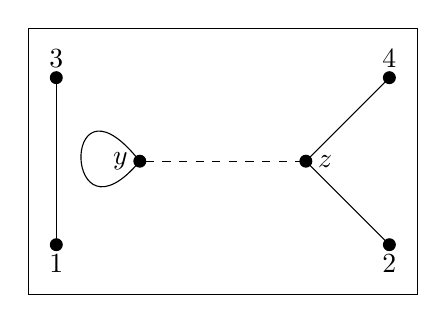
\begin{tikzpicture}[framed, baseline={(current bounding box.center)}]
                \begin{feynman}
                  \vertex [dot] (a) {} ;
                  \vertex [right = 6em of a, dot] (b) {} ;
                  \vertex [above left=of a, dot] (i1) {};
                  \vertex [below left =of a, dot] (i2) {};
                  \vertex [above right=of b,dot] (i3) {};
                  \vertex [below right=of b,dot] (i4) {};
                  \vertex (q) at (a);
                  \vertex (r) at (b);
                  \diagram * {
                    (i3) -- [plain] (b) -- [plain] (i4),
                    (a) -- [dashed] (b),
                    (i1)-- [plain] (i2),
%                    (a) -- [loop] node [left] {} (a),
                  (a) -- [out=130, in=230, loop, min distance=1.5cm] (q),
%                    (b) -- [out=50, in=-50, loop, min distance=1.5cm] (r),
                  };
                  \vertex [left = 0.7em of a] {$y$};
                  \vertex [right = 0.7em of b] {$z$};
                  \vertex [above= 0.7em of i1] {$3$};
                  \vertex [below= 0.7em of i2] {$1$};
                  \vertex [above = 0.7em of i3] {$4$};
                  \vertex [below = 0.7em of i4] {$2$};
                \end{feynman}
            \end{tikzpicture} }%$\qquad$

            \resizebox{.4\textwidth}{.1\textwidth}{
            \begin{tikzpicture}[framed, baseline={(current bounding box.center)}]
              \begin{feynman}
                \vertex [dot] (a) {} ;
                \vertex [right = 6em of a, dot] (b) {} ;
                \vertex [above left=of a, dot] (i1) {};
                \vertex [below left =of a, dot] (i2) {};
                \vertex [left=of i1,dot] (i3) {};
                \vertex [left=of i2,dot] (i4) {};
                \diagram * {
                  (i1) -- [plain] (i3),
                  (i2) -- [plain] (a) -- [plain] (i4),
                  (a) -- [dashed] (b),
%                  (a) -- [out=130, in=230, loop, min distance=1.5cm] (q),
%                    (a) -- [loop] node [left] {} (a),
                  (b) -- [out=50, in=-50, loop, min distance=1.5cm] (r),
                };
                \vertex [left = 0.7em of a] {$y$};
                \vertex [right = 0.7em of b] {$z$};
                \vertex [above= 0.7em of i1] {$4$};
                \vertex [below= 0.7em of i2] {$2$};
                \vertex [above = 0.7em of i3] {$3$};
                \vertex [below = 0.7em of i4] {$1$};
              \end{feynman}
            \end{tikzpicture} }%$\qquad$
            \resizebox{.4\textwidth}{.1\textwidth}{
            \begin{tikzpicture}[framed, baseline={(current bounding box.center)}]
              \begin{feynman}
                \vertex [dot] (a) {} ;
                \vertex [right = 6em of a, dot] (b) {} ;
                \vertex [above left=of a, dot] (i1) {};
                \vertex [below left =of a, dot] (i2) {};
                \vertex [left=of i1,dot] (i3) {};
                \vertex [left=of i2,dot] (i4) {};
                \diagram * {
                  (i4) -- [plain] (i2),
                  (i1) -- [plain] (a) -- [plain] (i3),
                  (a) -- [dashed] (b),
%                  (a) -- [out=130, in=230, loop, min distance=1.5cm] (q),
%                    (a) -- [loop] node [left] {} (a),
                  (b) -- [out=50, in=-50, loop, min distance=1.5cm] (r),
                };
                \vertex [left = 0.7em of a] {$y$};
                \vertex [right = 0.7em of b] {$z$};
                \vertex [above= 0.7em of i1] {$4$};
                \vertex [below= 0.7em of i2] {$2$};
                \vertex [above = 0.7em of i3] {$3$};
                \vertex [below = 0.7em of i4] {$1$};
              \end{feynman}
            \end{tikzpicture} }
          %$\qquad$

            \resizebox{.4\textwidth}{.1\textwidth}{
            \begin{tikzpicture}[framed, baseline={(current bounding box.center)}]
              \begin{feynman}
                \vertex [dot] (a) {} ;
                \vertex [right = 6em of a, dot] (b) {} ;
                \vertex [above left=of a, dot] (i1) {};
                \vertex [below left =of a, dot] (i2) {};
                \vertex [left=of i1,dot] (i3) {};
                \vertex [left=of i2,dot] (i4) {};
                \diagram * {
                  %(i1) -- [plain] (i4),
                  %(i2) -- [plain] (i3),
                  (a) -- [dashed] (b),
                  (i1) -- [plain] (a) -- [plain] (i4);
%                  (a) -- [out=130, in=230, loop, min distance=1.5cm] (q),
%                    (a) -- [loop] node [left] {} (a),
                  (b) -- [out=50, in=-50, loop, min distance=1.5cm] (r),
                };
                \path [name path=line 1] (a) -- (i4);
                \path [name path=line 2] (i2) -- (i3);
                \path [name intersections={of = line 1 and line 2}];
                \coordinate (S)  at (intersection-1);
                \path[name path=circle] (S) circle(0.2);
                \path [name intersections={of = circle and line 2}];
                \coordinate (K1)  at (intersection-1);
                \coordinate (K2)  at (intersection-2);
                \draw (i2) -- (K2);
                \draw (K1) -- (i3);
                \tkzDrawArc[color=black](S,K2)(K1);
                \vertex [left = 0.7em of a] {$y$};
                \vertex [right = 0.7em of b] {$z$};
                \vertex [above= 0.7em of i1] {$4$};
                \vertex [below= 0.7em of i2] {$2$};
                \vertex [above = 0.7em of i3] {$3$};
                \vertex [below = 0.7em of i4] {$1$};
              \end{feynman}
            \end{tikzpicture} %$\qquad $
          }
            \resizebox{.4\textwidth}{.1\textwidth}{
            \begin{tikzpicture}[framed, baseline={(current bounding box.center)}]
              \begin{feynman}
                \vertex [dot] (a) {} ;
                \vertex [right = 6em of a, dot] (b) {} ;
                \vertex [above left=of a, dot] (i1) {};
                \vertex [below left =of a, dot] (i2) {};
                \vertex [left=of i1,dot] (i3) {};
                \vertex [left=of i2,dot] (i4) {};
                \diagram * {
                  (i1) -- [plain] (i4),
                  (i2) -- [plain] (a),
                  %(i2) -- [plain] (i3),
                  (a) -- [dashed] (b),
%                  (a) -- [out=130, in=230, loop, min distance=1.5cm] (q),
%                    (a) -- [loop] node [left] {} (a),
                  (b) -- [out=50, in=-50, loop, min distance=1.5cm] (r),
                };
                \path [name path=line 1] (i1) -- (i4);
                \path [name path=line 2] (i3) -- (a);
                \path [name intersections={of = line 1 and line 2}];
                \coordinate (S)  at (intersection-1);
                \path[name path=circle] (S) circle(0.2);
                \path [name intersections={of = circle and line 2}];
                \coordinate (K1)  at (intersection-1);
                \coordinate (K2)  at (intersection-2);
                \draw (a) -- (K2);
                \draw (K1) -- (i3);
                \tkzDrawArc[color=black](S,K2)(K1);
                \vertex [left = 0.7em of a] {$y$};
                \vertex [right = 0.7em of b] {$z$};
                \vertex [above= 0.7em of i1] {$4$};
                \vertex [below= 0.7em of i2] {$2$};
                \vertex [above = 0.7em of i3] {$3$};
                \vertex [below = 0.7em of i4] {$1$};
              \end{feynman}
            \end{tikzpicture}% \\ 
          }

            \resizebox{.4\textwidth}{.1\textwidth}{
            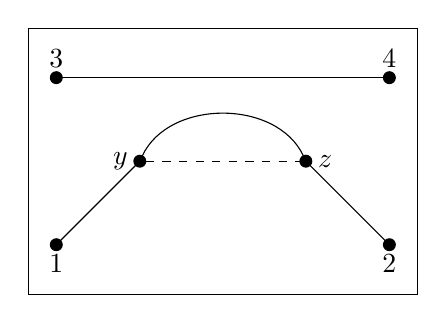
\begin{tikzpicture}[framed, baseline={(current bounding box.center)}]
              \begin{feynman}
                \vertex [dot] (a) {} ;
                \vertex [right = 6em of a, dot] (b) {} ;
                \vertex [above left=of a, dot]  (i1) {};
                \vertex [below left =of a, dot] (i2) {};
                \vertex [above right=of b, dot] (i3) {};
                \vertex [below right=of b, dot] (i4) {};
                \diagram * {
                  (i1) -- [plain] (i3),
                  (i2) -- [plain] (a),
%                  (i3) -- [plain] (b),
                  (i4) -- [plain] (b),
                  (a) -- [dashed] (b),
                  (a) -- [out=65, in=115, min distance=0.5cm] (b),% -- [out=225, in=-45, min distance=0.5cm] (a),
                };
                \vertex [left = 0.7em of a] {$y$};
                \vertex [right = 0.7em of b] {$z$};
                \vertex [above= 0.7em of i1] {$3$};
                \vertex [below= 0.7em of i2] {$1$};
                \vertex [above = 0.7em of i3] {$4$};
                \vertex [below = 0.7em of i4] {$2$};
              \end{feynman}
            \end{tikzpicture} }%$\qquad \phantom{=} \quad$
            \resizebox{.4\textwidth}{.1\textwidth}{
            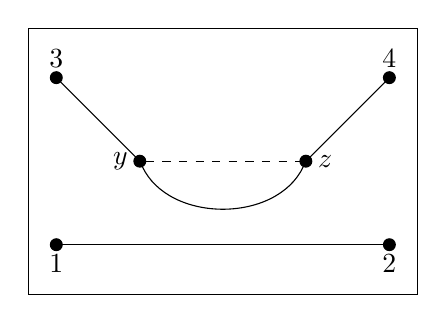
\begin{tikzpicture}[framed, baseline={(current bounding box.center)}]
              \begin{feynman}
                \vertex [dot] (a) {} ;
                \vertex [right = 6em of a, dot] (b) {} ;
                \vertex [above left=of a, dot]  (i1) {};
                \vertex [below left =of a, dot] (i2) {};
                \vertex [above right=of b, dot] (i3) {};
                \vertex [below right=of b, dot] (i4) {};
                \diagram * {
                  (i2) -- [plain] (i4),
                  (i1) -- [plain] (a),
%                  (i3) -- [plain] (b),
                  (i3) -- [plain] (b),
                  (a) -- [dashed] (b),
                  (a) -- [out=-65, in=-115, min distance=0.5cm] (b),% -- [out=225, in=-45, min distance=0.5cm] (a),
                };
                \vertex [left = 0.7em of a] {$y$};
                \vertex [right = 0.7em of b] {$z$};
                \vertex [above= 0.7em of i1] {$3$};
                \vertex [below= 0.7em of i2] {$1$};
                \vertex [above = 0.7em of i3] {$4$};
                \vertex [below = 0.7em of i4] {$2$};
              \end{feynman}
            \end{tikzpicture}}
            \resizebox{.4\textwidth}{.1\textwidth}{
            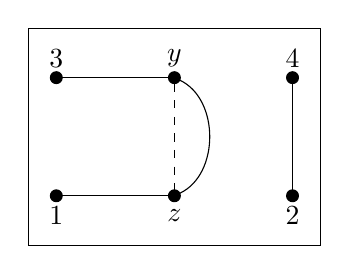
\begin{tikzpicture}[framed, baseline={(current bounding box.center)}]
              \begin{feynman}
                \vertex [dot] (a) {} ;
                \vertex [below = of a, dot] (b) {} ;
                \vertex [left=of a, dot]  (i1) {};
                \vertex [left =of b, dot] (i2) {};
                \vertex [right=of a, dot] (i3) {};
                \vertex [right=of b, dot] (i4) {};
                \diagram * {
                  (i4) -- [plain] (i3),
                  (a) -- [plain] (i1),
%                  (i3) -- [plain] (b),
                  (i2) -- [plain] (b),
                  (a) -- [dashed] (b),
                  (a) -- [out=-25, in=25, min distance=0.5cm] (b),% -- [out=225, in=-45, min distance=0.5cm] (a),
                };
                \vertex [above = 0.7em of a] {$y$};
                \vertex [below = 0.7em of b] {$z$};
                \vertex [above= 0.7em of i1] {$3$};
                \vertex [below= 0.7em of i2] {$1$};
                \vertex [above = 0.7em of i3] {$4$};
                \vertex [below = 0.7em of i4] {$2$};
              \end{feynman}
            \end{tikzpicture}
          }
            %$\qquad \phantom{=} \quad$
            \resizebox{.4\textwidth}{.1\textwidth}{
            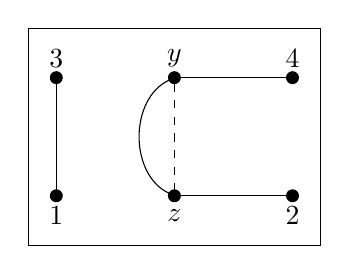
\begin{tikzpicture}[framed, baseline={(current bounding box.center)}]
              \begin{feynman}
                \vertex [dot] (a) {} ;
                \vertex [below = of a, dot] (b) {} ;
                \vertex [left=of a, dot]  (i1) {};
                \vertex [left =of b, dot] (i2) {};
                \vertex [right=of a, dot] (i3) {};
                \vertex [right=of b, dot] (i4) {};
                \diagram * {
                  (a) -- [plain] (i3),
                  (i1) -- [plain] (i2),
%                  (i3) -- [plain] (b),
                  (i4) -- [plain] (b),
                  (a) -- [dashed] (b),
                  (a) -- [out=-155, in=155, min distance=0.5cm] (b),% -- [out=225, in=-45, min distance=0.5cm] (a),
                };
                \vertex [above = 0.7em of a] {$y$};
                \vertex [below = 0.7em of b] {$z$};
                \vertex [above= 0.7em of i1] {$3$};
                \vertex [below= 0.7em of i2] {$1$};
                \vertex [above = 0.7em of i3] {$4$};
                \vertex [below = 0.7em of i4] {$2$};
              \end{feynman}
            \end{tikzpicture}
          }
            \resizebox{.4\textwidth}{.1\textwidth}{
            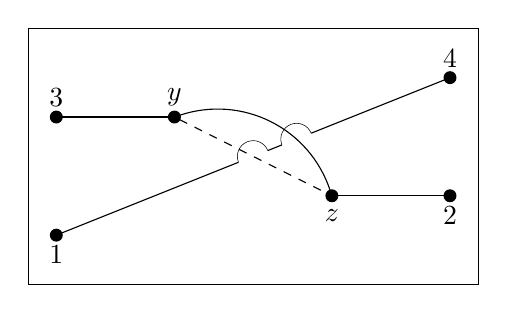
\begin{tikzpicture}[framed, baseline={(current bounding box.center)}]
              \begin{feynman}
                \vertex [dot] at (0,0) (a) {} ;
                \vertex [dot] at (2, -1) (b) {} ;
                \vertex [left=of a, dot]  (i1) {};
                \vertex [below=of i1, dot] (i2) {};
                \vertex [right=of b, dot] (i4) {};
                \vertex [above=of i4, dot] (i3) {};
                \diagram * {
%                  (i2) -- [plain] (i3),
                  (a) -- [plain] (i1),
%                  (i3) -- [plain] (b),
                  (i4) -- [plain] (b),
%                  (a) -- [dashed] (b),
                  (a) -- [out=18.4349, in=108.4349, min distance=0.5cm] (b),% -- [out=225, in=-45, min distance=0.5cm] (a),
                };
                \vertex [above = 0.7em of a] {$y$};
                \vertex [below = 0.7em of b] {$z$};
                \vertex [above= 0.7em of i1] {$3$};
                \vertex [below= 0.7em of i2] {$1$};
                \vertex [above = 0.7em of i3] {$4$};
                \vertex [below = 0.7em of i4] {$2$};

                \draw[dashed, name path=line 1] (a) -- (b);
                \path [name path=line 2] (i3) -- (i2);
                \path [name path=line 3] (a) to[out=18.4349, in=108.4349, min distance=0.5cm] (b);
                \path [name intersections={of = line 1 and line 2}];
                \coordinate (S)  at (intersection-1);
                \path[name path=circle] (S) circle(0.2);
                \path [name intersections={of = circle and line 2}];
                \coordinate (K1)  at (intersection-1);
                \coordinate (K2)  at (intersection-2);
                \tkzDrawArc[color=black](S,K1)(K2);

                \path [name intersections={of = line 2 and line 3}];
                \coordinate (S2)  at (intersection-1);
                \path[name path=circle] (S2) circle(0.2);
                \path [name intersections={of = circle and line 2}];
                \coordinate (K3)  at (intersection-1);
                \coordinate (K4)  at (intersection-2);

                \tkzDrawArc[color=black](S2,K3)(K4);
                \draw (i3) -- (K3);
                \draw (K4) -- (K1);
                \draw (K2) -- (i2);
              \end{feynman}
            \end{tikzpicture}
          }
            %$\qquad \phantom{=} \quad$
            \resizebox{.4\textwidth}{.1\textwidth}{
            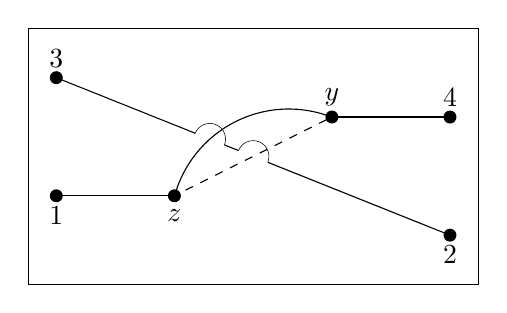
\begin{tikzpicture}[framed, baseline={(current bounding box.center)}]
              \begin{feynman}
                \vertex [dot] at (0,0) (a) {} ;
                \vertex [dot] at (-2,-1) (b) {} ;
                \vertex [left =of b, dot] (i2) {};
                \vertex [above=of i2, dot]  (i1) {};
                \vertex [right=of a, dot] (i3) {};
                \vertex [below=of i3, dot] (i4) {};
%                \draw[] (b) to[out=71.565, in=161.565, min distance=0.5cm] (i1);%[out=71.565, in=161.565, min distance=0.5cm] (c);% -- [out=225, in=-45, min distance=0.5cm] (a),
                \diagram * {
                  (a) -- [plain] (i3),
%                  (i1) -- [plain] (i4),
%                  (i3) -- [plain] (b),
                  (i2) -- [plain] (b),
%                  (a) -- [dashed] (b),
                  (b) -- [out=71.565, in=161.565, min distance=0.5cm] (a),% -- [out=225, in=-45, min distance=0.5cm] (a),
                };
                \vertex [above = 0.7em of a] {$y$};
                \vertex [below = 0.7em of b] {$z$};
                \vertex [above= 0.7em of i1] {$3$};
                \vertex [below= 0.7em of i2] {$1$};
                \vertex [above = 0.7em of i3] {$4$};
                \vertex [below = 0.7em of i4] {$2$};

                \draw[dashed, name path=line 1] (a) -- (b);
                \path [name path=line 2] (i4) -- (i1);
                \path [name path=line 3] (b) to[out=71.565, in=161.565, min distance=0.5cm] (a);
                \path [name intersections={of = line 1 and line 2}];
                \coordinate (S)  at (intersection-1);
                \path[name path=circle] (S) circle(0.2);
                \path [name intersections={of = circle and line 2}];
                \coordinate (K1)  at (intersection-1);
                \coordinate (K2)  at (intersection-2);
                \tkzDrawArc[color=black](S,K2)(K1);

                \path [name intersections={of = line 2 and line 3}];
                \coordinate (S2)  at (intersection-1);
                \path[name path=circle] (S2) circle(0.2);
                \path [name intersections={of = circle and line 2}];
                \coordinate (K3)  at (intersection-1);
                \coordinate (K4)  at (intersection-2);

                \tkzDrawArc[color=black](S2,K4)(K3);
                \draw (i1) -- (K3);
                \draw (K4) -- (K1);
                \draw (K2) -- (i4);
              \end{feynman}
            \end{tikzpicture}
          }%\\
            \end{center}
          \item
            These are the only diagrams.
            \begin{center}            
            \end{center}
            \begin{center}
              \resizebox{.4\textwidth}{.1\textwidth}{
            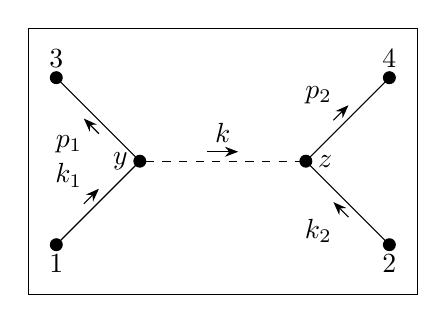
\begin{tikzpicture}[framed, baseline={(current bounding box.center)},
                arrowlabel/.style={
                  /tikzfeynman/momentum/.cd, % means that the following keys are read from the /tikzfeynman/momentum family
                  arrow shorten=#1,arrow distance=1.2mm
                },
                arrowlabel/.default=0.4
              ]
              \begin{feynman}
                \vertex [dot] (a) {} ;
                \vertex [right = 6em of a, dot] (b) {} ;
                \vertex [above left=of a, dot]  (i1) {};
                \vertex [below left =of a, dot] (i2) {};
                \vertex [above right=of b, dot] (i3) {};
                \vertex [below right=of b, dot] (i4) {};
                \diagram * {
                  (a) -- [plain, momentum={[arrowlabel]$p_1$}] (i1),
                  (i2) -- [plain, momentum={[arrowlabel]$k_1$}] (a),
                  (b) -- [plain, momentum={[arrowlabel]$p_2$}] (i3),
                  (i4) -- [plain, momentum={[arrowlabel]$k_2$}] (b),
                  (a) -- [dashed, momentum={[arrowlabel]$k$}] (b),
                };
                \vertex [left = 0.7em of a] {$y$};
                \vertex [right = 0.7em of b] {$z$};
                \vertex [above= 0.7em of i1] {$3$};
                \vertex [below= 0.7em of i2] {$1$};
                \vertex [above = 0.7em of i3] {$4$};
                \vertex [below = 0.7em of i4] {$2$};
              \end{feynman}
            \end{tikzpicture}
          }
          \resizebox{.4\textwidth}{.1\textwidth}{
            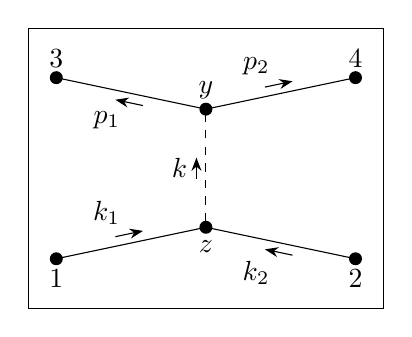
\begin{tikzpicture}[framed, baseline={(current bounding box.center)},
                arrowlabel/.style={
                  /tikzfeynman/momentum/.cd, % means that the following keys are read from the /tikzfeynman/momentum family
                  arrow shorten=#1,arrow distance=1.2mm
                },
                arrowlabel/.default=0.4
              ]
              \begin{feynman}
                \vertex [dot] at (0,0) (a) {} ;
                \vertex [dot] at (0, -1.5) (b) {} ;
                \vertex [dot] at (-1.9, 0.4)  (i1) {};
                \vertex [dot] at (-1.9, -1.9) (i2) {};
                \vertex [dot] at (1.9, 0.4) (i3) {};
                \vertex [dot] at (1.9, -1.9) (i4) {};
                \diagram * {
                  (a) -- [plain, momentum={[arrowlabel]$p_1$}] (i1),
                  (i2) -- [plain, momentum={[arrowlabel]$k_1$}] (b),
                  (a) -- [plain, momentum={[arrowlabel]$p_2$}] (i3),
                  (i4) -- [plain, momentum={[arrowlabel]$k_2$}] (b),
                  (b) -- [dashed, momentum={[arrowlabel]$k$}] (a),
                };
                \vertex [above= 0.7em of a] {$y$};
                \vertex [below= 0.7em of b] {$z$};
                \vertex [above= 0.7em of i1] {$3$};
                \vertex [below= 0.7em of i2] {$1$};
                \vertex [above = 0.7em of i3] {$4$};
                \vertex [below = 0.7em of i4] {$2$};
              \end{feynman}
            \end{tikzpicture}
          }
          \resizebox{.4\textwidth}{.1\textwidth}{
            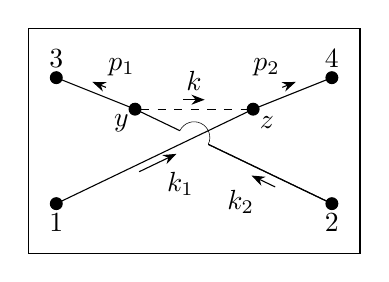
\begin{tikzpicture}[framed, baseline={(current bounding box.center)},
                arrowlabel/.style={
                  /tikzfeynman/momentum/.cd, % means that the following keys are read from the /tikzfeynman/momentum family
                  arrow shorten=#1,arrow distance=1.2mm
                },
                arrowlabel/.default=0.4,
                arrowlabelShort/.style={
                  /tikzfeynman/momentum/.cd, % means that the following keys are read from the /tikzfeynman/momentum family
                  arrow shorten=#1,arrow distance=0.9mm
                },
                arrowlabelShort/.default=0.4,
              ]
              \begin{feynman}
                \vertex [dot] at (0,0) (a) {} ;
                \vertex [dot] at (1.5,0) (b) {} ;
                \vertex [dot] at (-1, 0.4) (i1) {};
                \vertex [dot] at (-1, -1.2) (i2) {};
                \vertex [dot] at (2.5, 0.4) (i3) {};
                \vertex [dot] at (2.5, -1.2) (i4) {};
                \vertex [below left = 0.7em of a] {$y$};
                \vertex [below right = 0.7em of b] {$z$};
                \vertex [above= 0.7em of i1] {$3$};
                \vertex [below= 0.7em of i2] {$1$};
                \vertex [above = 0.7em of i3] {$4$};
                \vertex [below = 0.7em of i4] {$2$};

                \path [name path=line 1] (i2) -- (b);
                \path [name path=line 2] (i4) -- (a);
                \path [name intersections={of = line 1 and line 2}];
                \coordinate (S)  at (intersection-1);
                \path[name path=circle] (S) circle(0.2);
                \path [name intersections={of = circle and line 2}];
                \coordinate (K1)  at (intersection-1);
                \coordinate (K2)  at (intersection-2);
                \draw (i4) -- (K2);
                \draw (K1) -- (a);
                \tkzDrawArc[color=black](S,K2)(K1);

                \diagram * {
                  (i1) -- [plain, reversed momentum={[arrowlabel]$p_1$}] (a),
                  (b) -- [plain, reversed momentum={[arrowlabelShort]$k_1$}] (i2),
                  (b) -- [plain, momentum={[arrowlabel]$p_2$}] (i3),
                  (i4) -- [plain, momentum={[arrowlabel]$k_2$}] (K2),
                  (a) -- [dashed, momentum={[arrowlabel]$k$}] (b),
                };
              \end{feynman}
            \end{tikzpicture}
          }
            \end{center}
        \end{enumerate}
      \item
        The first set contains all possible diagrams with two vertices, the second set is a subset of the first that contains all connected diagrams withouth vacuum subdiagrams.
        The last diagram is a subset of the first two that only has the fully connected (and amputated) diagrams.
      \item
        I discussed this quesion with PA and we decided that this diagram has a symmetry factor of 8.\\
        \begin{center}
        \resizebox{.4\textwidth}{.1\textwidth}{
          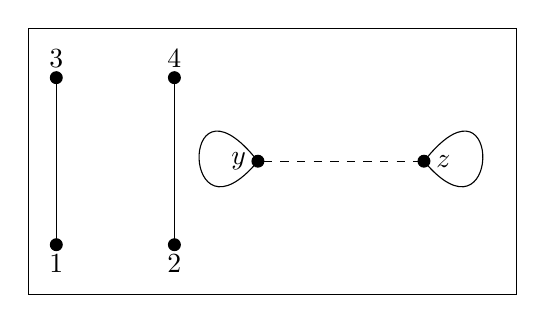
\begin{tikzpicture}[framed, baseline={(current bounding box.center)}]
            \begin{feynman}
              \vertex [dot] (a) {} ;
              \vertex [right = 6em of a, dot] (b) {} ;
              \vertex [above left=of a, dot] (i1) {};
              \vertex [below left =of a, dot] (i2) {};
              \vertex [left=of i1,dot] (i3) {};
              \vertex [left=of i2,dot] (i4) {};
              \vertex (q) at (a);
              \vertex (r) at (b);
              \diagram * {
                (i1) -- [plain] (i2),
                (i3) -- [plain] (i4),
                (a) -- [dashed] (b),
                (a) -- [out=130, in=230, loop, min distance=1.5cm] (q),
%                    (a) -- [loop] node [left] {} (a),
                (b) -- [out=50, in=-50, loop, min distance=1.5cm] (r),
              };
              \vertex [left = 0.7em of a] {$y$};
              \vertex [right = 0.7em of b] {$z$};
              \vertex [above= 0.7em of i1] {$4$};
              \vertex [below= 0.7em of i2] {$2$};
              \vertex [above = 0.7em of i3] {$3$};
              \vertex [below = 0.7em of i4] {$1$};
            \end{feynman}
          \end{tikzpicture} %$\qquad$
        }
          \end{center}

          The ends of the solid lines at $y$ (factor of two) and $z$ (factor of two) can be swapped, and vertices, $y$ and $z$, can be swapped (factor of two).
          The factor in front of the integral is:
          \begin{align*}
            & \frac{1}{2} \langle 0|\left(-i\frac{g}{2}\int d^4y \Phi(y)\phi^2(y)\right)\left(-i\frac{g}{2}\int dz \Phi(z)\phi^2(z)\right)|0\rangle \\
            = &- \frac{1}{8} g^2 \int d^4y \int dz\langle 0|\Phi(y)\phi^2(y) \Phi(z)\phi^2(z)|0\rangle
          \end{align*}
          The only Wick contraction is:\\

          \begin{equation*}
            \langle 0|
              \rnode{p1}{\phi}_1
              \rnode{p2}{\phi}_2
              \rnode{p3}{\phi}_3
              \rnode{p4}{\phi}_4
               \rnode{Py}{\Phi}_y \rnode{py1}{\phi}_y \rnode{py2}{\phi}_y \rnode{Pz}{\Phi}_z \rnode{pz1}{\phi}_z \rnode{pz2}{\phi}_z
               \ncbar[nodesep=0.5ex, arm=1ex, angle=90]{p1}{p3}
               \ncbar[nodesep=0.5ex, arm=1.5ex, angle=90]{p2}{p4}
               \ncbar[nodesep=0.5ex, arm=1ex, angle=90]{Py}{Pz}
               \ncbar[nodesep=0.5ex, arm=1.5ex, angle=90]{py1}{py2}
               %\naput{2}
               \ncbar[nodesep=0.5ex, arm=1ex, angle=90]{pz1}{pz2}
            |0\rangle
          \end{equation*}
          Thus the symmetry factor is given by:
          \begin{equation*}
            \frac{1}{8} = \frac{1}{S}
          \end{equation*}
          I did another two diagrams on my own to see if my understanding is correct, hupefully the first one is right.
          This diagram has a symmetry factor of $2$.
          \begin{center}
            \resizebox{.4\textwidth}{.1\textwidth}{
            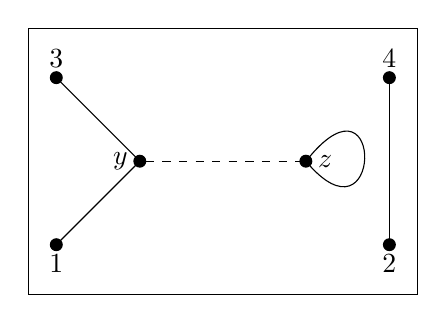
\begin{tikzpicture}[framed, baseline={(current bounding box.center)}]
                \begin{feynman}
                  \vertex [dot] (a) {} ;
                  \vertex [right = 6em of a, dot] (b) {} ;
                  \vertex [above left=of a, dot] (i1) {};
                  \vertex [below left =of a, dot] (i2) {};
                  \vertex [above right=of b,dot] (i3) {};
                  \vertex [below right=of b,dot] (i4) {};
                  \vertex (q) at (a);
                  \vertex (r) at (b);
                  \diagram * {
                    (i3) -- [plain] (i4),
                    (a) -- [dashed] (b),
                    (a)-- [plain] (i1),
                    (a)-- [plain] (i2),
%                    (a) -- [loop] node [left] {} (a),
                    (b) -- [out=50, in=-50, loop, min distance=1.5cm] (r),
                  };
                  \vertex [left = 0.7em of a] {$y$};
                  \vertex [right = 0.7em of b] {$z$};
                  \vertex [above= 0.7em of i1] {$3$};
                  \vertex [below= 0.7em of i2] {$1$};
                  \vertex [above = 0.7em of i3] {$4$};
                  \vertex [below = 0.7em of i4] {$2$};
                \end{feynman}
            \end{tikzpicture} }%$\qquad$
          \end{center}

          The Wick contractions are:\\

          \begin{equation*}
            \langle 0|
              \rnode{p1}{\phi}_1
              \rnode{p2}{\phi}_2
              \rnode{p3}{\phi}_3
              \rnode{p4}{\phi}_4
               \rnode{Py}{\Phi}_y \rnode{py1}{\phi}_y \rnode{py2}{\phi}_y \rnode{Pz}{\Phi}_z \rnode{pz1}{\phi}_z \rnode{pz2}{\phi}_z
               \ncbar[nodesep=0.5ex, arm=2ex, angle=90]{p1}{py1}
               \naput{2}
               \ncbar[nodesep=0.5ex, arm=1.5ex, angle=90]{p3}{py2}
               \ncbar[nodesep=0.5ex, arm=1ex, angle=90]{p2}{p4}
               \ncbar[nodesep=0.5ex, arm=1ex, angle=-90]{Py}{Pz}
               \ncbar[nodesep=0.5ex, arm=1ex, angle=90]{pz1}{pz2}
            |0\rangle
          \end{equation*}
          But since the labels are arbitrary, this diagram also corresponds to:\\

          \begin{equation*}
            \langle 0|
              \rnode{p1}{\phi}_1
              \rnode{p2}{\phi}_2
              \rnode{p3}{\phi}_3
              \rnode{p4}{\phi}_4
               \rnode{Py}{\Phi}_y \rnode{py1}{\phi}_y \rnode{py2}{\phi}_y \rnode{Pz}{\Phi}_z \rnode{pz1}{\phi}_z \rnode{pz2}{\phi}_z
               \ncbar[nodesep=0.5ex, arm=2ex, angle=90]{p1}{pz1}
               \naput{2}
               \ncbar[nodesep=0.5ex, arm=1.5ex, angle=90]{p3}{pz2}
               \ncbar[nodesep=0.5ex, arm=1ex, angle=90]{p2}{p4}
               \ncbar[nodesep=0.5ex, arm=1ex, angle=-90]{Py}{Pz}
               \ncbar[nodesep=0.5ex, arm=1ex, angle=-90]{py1}{py2}
            |0\rangle
          \end{equation*}
          There are thus four possible contractions for this Feynmann diagram:
          And hence:
          \begin{equation*}
            \frac{4}{8} = \frac{1}{2} = \frac{1}{S}
          \end{equation*}

          This diagram has a symmetry factor of $4$.
          \begin{center}
              \resizebox{.4\textwidth}{.1\textwidth}{
              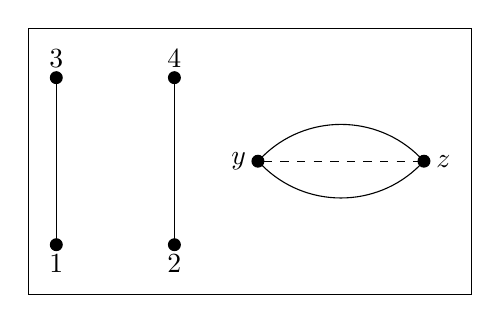
\begin{tikzpicture}[framed, baseline={(current bounding box.center)}]
                \begin{feynman}
                  \vertex [dot] (a) {} ;
                  \vertex [right = 6em of a, dot] (b) {} ;
                  \vertex [above left=of a, dot] (i1) {};
                  \vertex [below left =of a, dot] (i2) {};
                  \vertex [left=of i1,dot] (i3) {};
                  \vertex [left=of i2,dot] (i4) {};
                  \diagram * {
                    (i1) -- [plain] (i2),
                    (i3) -- [plain] (i4),
                    (a) -- [dashed] (b),
                    (a) -- [out=45, in=135, min distance=0.5cm] (b) -- [out=225, in=-45, min distance=0.5cm] (a),
                  };
                  \vertex [left = 0.7em of a] {$y$};
                  \vertex [right = 0.7em of b] {$z$};
                  \vertex [above= 0.7em of i1] {$4$};
                  \vertex [below= 0.7em of i2] {$2$};
                  \vertex [above = 0.7em of i3] {$3$};
                  \vertex [below = 0.7em of i4] {$1$};
                \end{feynman}
              \end{tikzpicture} 
            }
          \end{center}

          The Wick contractions are:\\

          \begin{equation*}
            \langle 0|
              \rnode{p1}{\phi}_1
              \rnode{p2}{\phi}_2
              \rnode{p3}{\phi}_3
              \rnode{p4}{\phi}_4
               \rnode{Py}{\Phi}_y \rnode{py1}{\phi}_y \rnode{py2}{\phi}_y \rnode{Pz}{\Phi}_z \rnode{pz1}{\phi}_z \rnode{pz2}{\phi}_z
               \ncbar[nodesep=0.5ex, arm=1ex, angle=90]{p1}{p3}
               \naput{2}
               \ncbar[nodesep=0.5ex, arm=1.5ex, angle=90]{p2}{p4}
               \ncbar[nodesep=0.5ex, arm=1ex, angle=-90]{Py}{Pz}
               \ncbar[nodesep=0.5ex, arm=2ex, angle=90]{py1}{pz1}
               \naput{2}
               \ncbar[nodesep=0.5ex, arm=1.5ex, angle=90]{py2}{pz2}
            |0\rangle
          \end{equation*}
          so that:
          \begin{equation*}
            \frac{2}{8} = \frac{1}{4} = \frac{1}{S}
          \end{equation*}
      \item
        I discussed the symmetry factors and Wick contractions with PA.

  \end{enumerate}
\end{enumerate}

\end{document}
